\section{Sequences}
In this section we use the notation \(\mathbb{K}\) to represent the field of \(\mathbb{R}\) respectively \(\mathbb{C}\) and specify otherwise.

\subsection{Definition \& Terminology}
\begin{definition}[Sequence]
   A map \(x: \mathbb{N} \to \mathbb{K}\) where we denote \(x_n := x(n)\).
\end{definition}
\begin{remark}[Notation]
   We denote a generic sequence as \((x_n)_{n \in \mathbb{N}}\).
   When we say ''\((x_n)_{n \in \mathbb{N}}\) is a sequence in \(\mathbb{K}\)`` we write \(x_n \in \mathbb{K}^\mathbb{N}\) where we mean that \(\forall n \in \mathbb{N}: x_n \in \mathbb{K}\).
\end{remark}
\begin{remark}[Intuition]
   A sequence viewed as a map is an \emph{enumeration}, so we can regard a sequence as an \emph{enumerated collection} of elements in \(\mathbb{K}\).
   \[(x_n)_{n \in \mathbb{N}} = x_1, x_2, \ldots, x_n\]
   Not to confuse with the enumerated set of points \(\{x_n \mid n \in \mathbb{N}\}\).
\end{remark}

\subsubsection{Convergence}
\begin{definition}[Convergent Sequence]\label{def:conv_seq}
   \(x_n \in \mathbb{K}^\mathbb{N}\) \emph{converges to} \(x \in \mathbb{K}\) iff
   \[\forall \varepsilon > 0~\exists n_\varepsilon \in \mathbb{N}: (\forall n \geq n_\varepsilon: |x_n - x| < \varepsilon)\]
\end{definition}
\begin{remark}[Intuition]
   \(x_n\) converges to \(x\), if after some index \(n_\varepsilon\) \emph{all} following \(x_n\) are closer to \(x\) than an arbitrarily chosen error margin \(\varepsilon\).
\end{remark}
\begin{remark}[Notation]
   If \(x_n\) converges to \(x\) we write
   \[x_n \xrightarrow{n \to \infty} x \qquad\text{or}\qquad \lim_{n \to \infty}(x_n) = x\]
\end{remark}
\begin{example}
   We regard the sequence \(x_n := \frac{1}{n}\) and show that \(\lim_{n \to \infty}(x_n) = 0\).

   Let \(\varepsilon > 0\) be arbitrary but fixed.
   According to the archimedes principle \(\exists n_\varepsilon \in \mathbb{N}: \frac{1}{n_\varepsilon} < \varepsilon\).

   Now since \(\forall n > n_\varepsilon: \frac{1}{n} < \frac{1}{n_\varepsilon}\), it follows that
   \[\forall \varepsilon > 0~\exists n_\varepsilon: \left(n > n_\varepsilon \implies \frac{1}{n} < \varepsilon\right)\]

   \begin{center}
      \begin{tikzpicture}[line cap=round, line join=round,>=triangle 45]
   \begin{axis}[
      x=2cm,y=2.5cm,
      axis lines=middle,
      ymajorgrids=true,
      xmajorgrids=true,
      xmin=-0.7,
      xmax=5.9,
      ymin=-0.3,
      ymax=1.5,
      xtick={0,1,...,5},
      ytick={0,1,...,2},
   ]

      \draw (-0.3,0.4) node {$\varepsilon = 0.3$};
      \draw [line width=2pt,color=red] (-1, 0.3) -- (5.5, 0.3);

      \draw (-0.3,0.1) node {$a = 0$};
      \draw [line width=2pt,color=blue] (-1, 0) -- (5.5, 0);

      \draw [fill=blue] (1,1) circle (2.5pt);
      \draw (1,1.1) node {$a_1$};

      \draw [fill=blue] (2,0.5) circle (2.5pt);
      \draw (2.,0.6) node {$a_2$};

      \draw [fill=blue] (3,0.33) circle (2.5pt);
      \draw (3.,0.43) node {$a_3$};

      \draw [fill=blue] (4,0.25) circle (2.5pt);
      \draw (4,0.35) node {$a_4$};

      \draw [fill=blue] (5,0.2) circle (2.5pt);
      \draw (5,0.3) node {$a_5$};
   \end{axis}
\end{tikzpicture}

   \end{center}
\end{example}

\subsubsection{Bounded \& Monotonic Sequences}
\begin{definition}[Bounded Sequence]
   A sequence \((x_n)_{n \in \mathbb{N}}\) is
   \[\text{bounded below} :\iff \exists b \in \mathbb{R}: (\forall n \in \mathbb{N}: b \leq x_n)\]
   \[\text{bounded above} :\iff \exists b \in \mathbb{R}: (\forall n \in \mathbb{N}: x_n \leq b)\]
   \[\text{bounded} :\iff \exists b \in \mathbb{R}_{>0}: (\forall n \in \mathbb{N}: |x_n| \leq b)\]
\end{definition}
\begin{remark}
   Since \(\lvert x_n \rvert < b \iff -b < x_n < b\) we see that \(x_n\) is \emph{bounded} if it is bounded above and below.
\end{remark}

\begin{theorem}[Convergent\(\implies\)Bounded]\label{thm:conv_bound}
   Every convergent sequence is bounded.
\end{theorem}
\begin{remark}
   The contraposition: ''Every unbounded sequence diverges``, is often more usefull.
\end{remark}

\begin{definition}[Monotonic Sequence]
   \(x_n \in \mathbb{R}^\mathbb{N}\) is
   \[\text{increasing} :\iff \forall n \in \mathbb{N}: x_n \leq x_{n+1}\]
   \[\text{decreasing} :\iff \forall n \in \mathbb{N}: x_n \geq x_{n+1}\]
\end{definition}
\begin{remark}[Terminology]
   If instead we have \(<\) or \(>\), we say \(x_n\) is \emph{strictly} monotonic.
\end{remark}
\begin{remark}[Tips]
   To prove that \(x_n\) is increasing, respectively decreasing we can show that
   \begin{enumerate}
      \item \(x_{n+1} = \ldots \geq x_n\) resp. \(x_{n+1} = \ldots \leq x_n\)
      \item \(\frac{x_{n+1}}{x_n} = \ldots \geq 1\) resp. \(\frac{x_{n+1}}{x_n} = \ldots < 1\)
      \item \(x_{n+1} - x_n = \ldots \geq 0\) resp. \(x_{n+1} - x_n = \ldots \leq 0\)
      \item For a recursive sequence we can use induction.
   \end{enumerate}
\end{remark}

\begin{theorem}[Monotonic \& Bounded Convergence]\label{thm:incr_bound_conv}
   If \(x_n \in \mathbb{R}^\mathbb{N}\) is
   \[\text{increasing and bounded above, then is} \quad \lim_{n \to \infty}(x_n) = \sup\{x_n \mid n \in \mathbb{N}\}\]
   \[\text{decreasing and bounded below, then is} \quad \lim_{n \to \infty}(x_n) = \inf\{x_n \mid n \in \mathbb{N}\}\]
\end{theorem}
\begin{example}
   Let \(x_0 := a \geq 1\) and \(x_{n+1} := \frac{1}{2} \left(x_n + \frac{a}{x_n}\right)\).
   We want to prove that \(\lim_{n \to \infty}(x_n) = \sqrt{a}\).

   First we prove that \(x_n\) is decreasing.
   \[x_{n+1} = \frac{1}{2} \left(x_n + \frac{a}{x_n}\right) = \frac{x_n}{2} \left(1 + \frac{a}{x_n^2}\right) \overset{x_n^2 \geq a}{\leq} \frac{x_n}{2} \left(1 + \frac{a}{a}\right) = x_n\]

   Now we show that \(x_n\) is bounded below by induction over \(n\)

   \emph{IB:} \(n = 0 \implies x_0 = a \geq \sqrt{a}\) holds since \(a \geq 1\).

   \emph{IH:} For some \(n \in \mathbb{N}\) holds \(x_n \geq \sqrt{a}\).

   \emph{IS:} Assume IH holds.
   \begin{equation*}
      \begin{split}
         x_{n+1} \geq \sqrt{a} & \iff \frac{1}{2} \left(x_n + \frac{a}{x_n}\right) \geq \sqrt{a} \iff x_n + \frac{a}{x_n} \geq 2 \sqrt{a}\\
                               & \iff x_n - 2\sqrt{a} \geq - \frac{a}{x_n} \iff x_n(x_n - 2\sqrt{a}) \geq -a
      \end{split}
   \end{equation*}
   but
   \[x_n(x_n - 2 \sqrt{a}) \overset{\text{IH}}{\geq} \sqrt{a}(\sqrt{a} - 2 \sqrt{a}) = -a\]
   So according to the induction axiom and IB, IH, IS follows that \(x_n\) is bounded below \(\forall n \in \mathbb{N}\).
\end{example}

\subsubsection{Improper Convergence}
\begin{definition}[Improper Convergence]
   Given \(x_n \in \mathbb{R}^\mathbb{N}\).
   \[\lim_{n \to \infty}(x_n) = \infty :\iff \forall M \in \mathbb{R}_{\geq 0}~\exists n_M \in \mathbb{N}: (\forall n \geq n_M: x_n > M)\]
   \[\lim_{n \to \infty}(x_n) = -\infty :\iff \forall M \in \mathbb{R}_{\geq 0}~\exists n_M \in \mathbb{N}: (\forall n \geq n_M: x_n < M)\]
\end{definition}
\begin{example}
   Let \(x_n := \log(n)\) and \(M \in \mathbb{R}\) be arbitrarily large.
   According to Archimedes principle \(\exists n_\varepsilon \in \mathbb{N}: n_\varepsilon \geq \lceil e^M\rceil\).
   Now let \(n > n_\varepsilon\), then
   \[\log(n) > \log(n_\varepsilon) \geq M\]
\end{example}
\begin{remark}
   \[\infty~\text{is an accumulation point of}~x_n :\iff \forall M \geq 0, n \in \mathbb{N}~\exists n_M \geq n: x_{n_M} > M\]
   \[-\infty~\text{is an accumulation point of}~x_n :\iff \forall M \geq 0, n \in \mathbb{N}~\exists n_M \geq n: x_{n_M} < -M\]
\end{remark}
\begin{example}
   \(x_n := (-1)^n \cdot n\) does not converge in \(\overline{R}\) but has the accumulation points \(\infty\) and \(-\infty\).
\end{example}

\begin{theorem}[Improper Limit]\label{thm:improper_limits}
   Every monotonic \(x_n \in \overline{\mathbb{R}}^\mathbb{N}\) converges and
   \[x_n~\text{increasing}~\implies \lim_{n \to \infty}(x_n) = \sup\{x_n \mid n \in \mathbb{N}\}\]
   \[x_n~\text{decreasing}~\implies \lim_{n \to \infty}(x_n) = \inf\{x_n \mid n \in \mathbb{N}\}\]
\end{theorem}
\begin{remark}
   Important to note here is that in contrast to \cref{thm:incr_bound_conv} we don't require \(x_n\) to be bounded.
\end{remark}

\subsection{Important Examples}
\begin{proposition}[Important Sequences]
   The following are important examples of sequences.

   \begin{enumerate}[label=\roman*, align=Center]
      \item Fibonacci Sequence
         \[x_0 := 1 \quad x_1 := 1 \qquad x_{n} := x_{n-1} + x_{n-2}\]
      \item \[\lim_{n \to \infty} \left(\frac{1}{n}\right) = 0\]
      \item \[\lim_{n \to \infty}(x^n) = \begin{cases}
               0 & x \in (-1; 1)\\
               1 & x = 1\\
               \pm\infty & x \in \mathbb{R}\setminus (-1;1)
         \end{cases}\]
      \item Let \(|x| < 1\) and \(r \in \mathbb{N}\)
         \[\lim_{n \to \infty}\big(n^r \cdot x^n\big) = 0\]
      \item \[\lim_{n \to \infty}(\sqrt[n]{n}) = 1\]
      \item \(\forall r \in \mathbb{R}_{>0}\)
         \[\lim_{n \to \infty}(\sqrt[n]{r}) = 1\]
      \item \(\forall s \in \mathbb{R}_{>0}\)
         \[\lim_{n \to \infty}(\sqrt[n]{n^s}) = 1\]
      \item \[\lim_{n \to \infty}\big(\sqrt[n]{n!}\big) = \infty\]
      \item Let \(x_k := \sum_{n=0}^k \frac{1}{n!}\)
         \[\lim_{k \to \infty}(x_k) = e\]
      \item \[\lim_{n \to \infty}\left(1 + \frac{1}{n}\right)^n = e\]
      \item \(\forall z \in \mathbb{C}\)
         \[\lim_{n \to \infty}\left(1 + \frac{z}{n}\right)^n = e^z\]
      \item \[\lim_{n \to \infty}\left(\frac{n}{\sqrt[n]{n!}}\right) = e\]
      \item \[\lim_{n \to \infty}\big(n \cdot (\sqrt[n]{a} - 1)\big) = \ln(a)\]
      \item
         \[\lim_{n \to \infty}\left(\frac{n!}{n^n}\right) = 0\]
   \end{enumerate}
\end{proposition}
\begin{remark}
   (ii) means that the sequence \(x^n\) converges faster to 0 than any other power of \(n\).
\end{remark}
\begin{proof}[Proof (i)]
   Suppose \((x_n)\) converges, i.e. \(\lim_{n \to \infty} x^n = \tilde{x}\), then is
   \[\tilde{x} = \lim_{n \to \infty} x^n = \lim_{n \to \infty} x^{(n+1)} = \lim_{n \to \infty} (x \cdot x^n) = x \cdot \lim_{n \to \infty} x^n = x \cdot \tilde{x}\]
   where \(\tilde{x} = x \cdot \tilde{x}\) gives us two cases.

   \textbf{Case 1:} \(x = 1\) and \(\tilde{x}\) arbitrary is directly (ii), which is trivial since \(\lim_{n \to \infty} 1^n = \lim_{n \to \infty} 1 = 1\).

   \textbf{Case 2:} \(\tilde{x} = 0\) and \(x\) arbitrary.

   \textbf{Case 2.1:} \(|x| < 1\) implies that \(x = \frac{a}{b}\) with \(a < b\), so we regard \(|x_n| = |x^n| = |x|^n\)
   \[\frac{|x_{n+1}|}{|x_n|} = \frac{\left|\frac{a}{b}\right|^{n+1}}{\left|\frac{a}{b}\right|^n} = \frac{|a|^{n+1}\cdot|b|^n}{|a|^n\cdot|b|^{n+1}} = \left|\frac{a}{b}\right| < 1\]
   hence \((|x_n|)\) is decreasing and since \(\forall n \in \mathbb{N}: 0 \leq |x_n|\) also bounded below.
   So \(|x_n| \xrightarrow{n \to \infty} 0\), according to \cref{thm:incr_bound_conv} and thus \(\lim_{n \to \infty} x_n = 0\).

   \textbf{Case 2.2:} \(|x| = 1\) but \(x \neq 1\).
   Suppose \((x_n)\) converges, then \(\lim_{n \to \infty} x_n = \tilde{x} = 0\) by assumption.
   So according to \cref{lem:zero_seq} (i) \(\lim_{n \to \infty} |x_n| = 0\).
   But this is a contradiction to \(|x| = 1\), hence \((x_n)\) diverges.

   \textbf{Cases 2.3:} \(|x| > 1 \implies \left(\frac{1}{|x|}\right)^n \xrightarrow{n \to \infty} 0\)
   This means that
   \[\forall \varepsilon > 0~\exists n_\varepsilon \in \mathbb{N}: \left(\forall n > n_\varepsilon: \frac{1}{|x^n|} < \varepsilon\right)\]
   hence \((x_n)\) is unbounded below and thus diverges according to \cref{thm:conv_bound}.
\end{proof}
\begin{proof}[Proof (ii)]
   The case where \(x = 0\) is trivial, so assume w.l.o.g. \(x \neq 1\).
   We regard \(x_n := n^r \cdot |x|^n\), then \(x_n > 0\) and
   \[\frac{x_{n+1}}{x_n} = \frac{(n+1)^r \cdot |x|^{n+1}}{n^r \cdot |x|^n} = |x| \left(\frac{n+1}{n}\right)^r = |x| \left(1 + \frac{1}{n}\right)^r \xrightarrow{n \to \infty} |x|\]
   since \(\left(1 + \frac{1}{n}\right)^r \xrightarrow{n \to \infty} 1\).

   Now let \(\alpha \in \big(|x|; 1\big)\), then
   \[\exists n_0 \in \mathbb{N}~\forall n > n_0: \left(\frac{x_{n+1}}{x_n} - \alpha = \left|\frac{x_{n+1}}{x_n} - \alpha\right| < \alpha - |x| \implies \frac{x_{n+1}}{x_n} < \alpha  \implies x_{n+1} < \alpha \cdot x_n\right)\]
   So by induction \(\forall n > n_0: x_n \leq x_{n_0} \cdot \alpha^{n - n_0}\), hence
   \[|n^r \cdot x^n| = x_n \leq x_{n_0} \cdot \alpha^{n-n_0} \xrightarrow{n \to \infty} 0\]
   So according to \cref{lem:zero_seq} (iii) is \(n^rx^n \to 0\).
\end{proof}

\subsection{Calculation Rules}
\begin{definition}[Zero Sequence]
   \((x_n)_{n \in \mathbb{N}}\) where \(\lim_{n \to \infty}(x_n) = 0\).
\end{definition}

\begin{proposition}[Zero Sequence Rules]\label{lem:zero_seq}
   Let \((x_n)_{n \in \mathbb{N}}\) and let \((y_n)_{n \in \mathbb{N}}\) be a zero sequence, then
   \begin{enumerate}[label=\roman*, align=Center]
      \item \[\lim_{n \to \infty}(x_n) = x \iff \lim_{n \to \infty} (x_n - x) = 0\]
      \item \[\lim_{n \to \infty}(x_n) = 0 \iff \lim_{n \to \infty}\big(\lvert x_n\rvert\big) = 0\]
      \item \[x_n~\text{bounded} \implies \lim_{n \to \infty} (x_n \cdot y_n) = 0\]
      \item \[\exists n_0 \in \mathbb{N}: (\forall n \geq n_0: |x_n| \leq y_n) \implies \lim_{n \to \infty}(x_n) = 0\]
   \end{enumerate}
\end{proposition}

\begin{proposition}[Sequence Limit Rules]\label{pro:seq_limit_rules}
   Let \(c \in \mathbb{K}\) and suppose \(x_n \xrightarrow{n \to \infty} x\), \(y_n \xrightarrow{n \to \infty} y\), then
   \begin{enumerate}[label=\roman*, align=Center]
      \item \[\lim_{n \to \infty}(c \cdot x_n) = c \cdot x\]
      \item \[\lim_{n \to \infty}(x_n \pm y_n) = x \pm y\]
      \item \[\lim_{n \to \infty}(x_n \cdot y_n) = x \cdot y\]
      \item If \(y \neq 0\) and \(\forall n \in \mathbb{N}: y_n \neq 0\), then
         \[\lim_{n \to \infty} \left(\frac{x_n}{y_n}\right) = \frac{x}{y}\]
      \item \[\lim_{n \to \infty}\big(\lvert x_n\rvert\big) = \lvert x \rvert\]
      \item If \(\forall n \in \mathbb{N}: x_n \geq 0\)
         \[\lim_{n \to \infty} \left(x_n^{\frac{p}{q}}\right) = x^{\frac{p}{q}} \qquad\text{with}~p \in \mathbb{Z}, q \in \mathbb{Z} \setminus \{0\}: \]
   \end{enumerate}
\end{proposition}
\begin{remark}
   From (vi) follows in particular that
   \[\lim_{n \to \infty}(x_n^{-1}) = \left(\lim_{n \to \infty}(x_n)\right)^{-1}\]
\end{remark}

\begin{proposition}\label{pro:limit_comp}
   Let \(x_n, y_n \in \mathbb{R}^\mathbb{N}\) where for infinite \(n \in \mathbb{N}: x_n \leq y_n\).
   \[\lim_{n \to \infty}(x_n) \leq \lim_{n \to \infty}(y_n)\]
\end{proposition}
\begin{remark}
   \(x_n := \frac{1}{n}\) and \(y_n := -\frac{1}{n}\) show that \(\forall n \in \mathbb{N}: x_n > y_n\) does not imply \(\lim_{n \to \infty} x_n > \lim_{n \to \infty} y_n\).
\end{remark}

\begin{proposition}[Sandwich Sequence]\label{pro:sandwich_seq}
   Let \(x_n, y_n, z_n \in \mathbb{R}^\mathbb{N}\) with \(\lim(x_n) = \lim(z_n) = y\).
   \[\exists n_0 \in \mathbb{N}:(\forall n > n_0: x_n \leq y_n \leq z_n) \implies \lim_{n \to \infty}(y_n) = y\]
\end{proposition}
\begin{example}
   Let \(y_n := \frac{\sin(n)}{n}\), we prove that \(\lim_{n \to \infty}(y_n) = 0\).
   First Note that \(\forall n \in \mathbb{N}\),
   \[-1 \leq \sin(x) \leq 1 \implies -\frac{1}{n} \leq \frac{\sin(x)}{n} \leq \frac{1}{n}\]
   So let \(x_n = -\frac{1}{n}\) and \(z_n = \frac{1}{n}\), where we know that \(\lim_{n \to \infty}(x_n) = \lim_{n \to \infty}(z_n) = 0\), thus
   \[\forall n \in \mathbb{N}: x_n \leq y_n \leq z_n \implies \lim_{n \to \infty}\left(\frac{\sin(n)}{n}\right) = 0\].
\end{example}

\begin{theorem}[Improper Convergence Rules]
   Let \(x_n \in \mathbb{R}^\mathbb{N}\)
   \begin{enumerate}[label=\roman*, align=Center]
      \item \[\lim_{n \to \infty}(x_n) = \pm\infty \implies \lim_{n \to \infty}\left(\frac{1}{x_n}\right) = 0\]
      \item \[\lim_{n \to \infty}(x_n) = 0~\text{and}~x_n > 0~\text{for almost all}~n \implies \lim_{n \to \infty}\left(\frac{1}{x_n}\right) = \infty\]
      \item \[\lim_{n \to \infty}(x_n) = 0~\text{and}~x_n < 0~\text{for almost all}~n \implies \lim_{n \to \infty}\left(\frac{1}{x_n}\right) = -\infty\]
   \end{enumerate}
\end{theorem}

\newpage

\subsection{Cauchy Sequences}
\begin{definition}[Cauchy Sequence]
   A sequence \((x_n)_{n \in \mathbb{N}}\) where
   \[\forall \varepsilon > 0~\exists n_\varepsilon \in \mathbb{N}: (\forall n, m > n_\varepsilon: \lvert x_n - x_m\rvert < \varepsilon)\]
\end{definition}
\begin{remark}[Intuition]
   In other words, given any small positive distance, almost all elements of the sequence are less than that given distance from each other.
\end{remark}
\begin{remark}[Tips]
   The \emph{cauchy condition} can be restated as
   \[\forall n, m > n_\varepsilon: |x_m - x_n| < \varepsilon \iff \forall m > n \geq n_\varepsilon: |x_m - x_n| < \varepsilon\]
   and also
   \[|x_m - x_n| = |(x_m - x) + (x - x_n)| \leq |x_m - x| + |x_n - x| < \varepsilon\]
\end{remark}

\begin{theorem}[Cauchy\(\implies\)Bounded]\label{thm:cauchy_bound}
   Every Cauchy sequence is bounded.
\end{theorem}

\begin{theorem}[Cauchy\(\iff\)Convergent]\label{thm:cauchy_crit_seq}
   Let \((x_n)_{n \in \mathbb{N}}\), then
   \[x_n~\text{is convergent} \iff x_n~\text{is a cauchy sequence}\]
\end{theorem}
\begin{remark}
   \(\implies\) holds always but \(\impliedby\) holds only if \(x_n \in \mathbb{K}\).
\end{remark}

\subsection{Subsequences \& Accumulation Points}
\begin{definition}[Subsequence]
   Given \((x_n)_{n \in \mathbb{N}}\) and \(\phi: \mathbb{N} \to \mathbb{N}\) strictly increasing
   \[(x_{n_k})_{k \in \mathbb{N}} := (x_{\phi(k)})_{k \in \mathbb{N}}\]
\end{definition}
\begin{example}
   Let \(x_n := n = 1, 2, 3, \ldots\).
   \[\begin{drcases}
         x: \mathbb{N} \to X \quad\text{where}\quad n \mapsto n \\
         \phi: \mathbb{N} \to \mathbb{N} \quad\text{where}\quad n \mapsto 2n
   \end{drcases} x \circ \phi: \mathbb{N} \to \mathbb{N} \to X\]
   \[x_1 = x(1) = 1 \qquad x_2 = x(2) = 2 \qquad x_3 = a(3) = 3 \qquad \ldots\]
   \[x_{n_1} = x\big(\phi(1)\big) = x(2) = 2 \qquad x_{n_2} = x\big(\phi(2)\big) = x(4) = 4 \qquad x_{n_3} = x\big(\phi(3)\big) = x(6) = 6\]
   We can write the subsequence in terms of the index of \(x_n\), without the subindices \(n_j\)
   \[x_{2n} = x_2, x_4, x_6, \ldots = 2, 4, 6, \ldots\]
\end{example}
\begin{example}
   Let \(x_n := (-1)^n\), then we see that
   \[x_{2n} = (-1)^{2n} = \big((-1)^2\big)^n = 1^n = 1\]
   \[x_{2n+1} = (-1)^{2n+1} = \big((-1)^2\big)^n \cdot (-1)^1 = 1^n \cdot (-1) = -1\]
\end{example}

\begin{theorem}\label{thm:all_subseq_conv}
   Let \((x_n)_{n \in \mathbb{N}}\), then
   \[\lim_{n \to \infty}(x_n) = x \iff \forall (x_{n_k})_{k \in \mathbb{N}}: \lim_{k \to \infty}(x_{n_k}) = x\]
\end{theorem}

\begin{theorem}\label{thm:cp_iff_subseq}
   Let \((x_n)_{n \in \mathbb{N}}\), then
   \[x~\text{is accumulation point of}~x_n \iff \exists (x_{n_k})_{k \in \mathbb{N}}: \lim_{k \to \infty}(x_{n_k}) = x\]
\end{theorem}

\begin{definition}[Accumulation Point]
   \(x \in \mathbb{K}\) is an \emph{accumulation point} of \(x_n \in \mathbb{K}^\mathbb{N}\) iff
   \[\forall \varepsilon > 0: \exists~\text{an infinite}~N_{\varepsilon} \subset \mathbb{N}: (\forall n \in N_\varepsilon: |x_n - x| < \varepsilon)\]
\end{definition}
\begin{example}
   Following some examples of sequences and their accumulation points.
   \begin{table}[h]\label{tbl:example_accumulation_points}
      \begin{center}
         \begin{tabular}{|c|c|}
            \hline
            Sequence \(x_n\)              & Accumulation Points        \\\hline
            \(a\)                         & \(a\)                      \\
            \(\frac{1}{n}\)               & \(0\)                      \\
            \((-1)^n\)                    & \(-1, 1\)                  \\
            \(i^n\)                       & \(-1, 1, -i, i\)           \\
            \(n\)                         & None                       \\
            Fibonacci                     & None                       \\
            Enumeration of \(\mathbb{Q}\) & Every \(a \in \mathbb{R}\) \\\hline
         \end{tabular}
      \end{center}
      % \caption{Examples of Accumulation Points}
   \end{table}
\end{example}

\begin{theorem}
   Let \(x_n \in \mathbb{K}^\mathbb{N}\) and \(x \in \mathbb{K}\), then is
   \[x~\text{an accumulation point of}~x_n \iff \forall \varepsilon > 0: (\forall n \in \mathbb{N}~\exists m \geq n: |x_m - x| < \varepsilon)\]
\end{theorem}

\begin{theorem}[Bolzano-Weierstrass]\label{thm:bolzano}
   Every bounded sequence in \(\mathbb{K}\) has at least one accumulation point.
\end{theorem}

\begin{theorem}
   Let \((x_n)_{n \in \mathbb{N}}\) such that \(\lim_{n \to \infty} x_n = x\), then
   \begin{enumerate}[label=\roman*, align=Center]
      \item \(x\) is the only accumulation point of \(x_n\)
      \item \(x\) is unique
   \end{enumerate}
\end{theorem}
\begin{remark}
   Note that the converse is in general false, e.g. \(\frac{1}{2}, 2, \frac{1}{3}, 3, \frac{1}{4}, 4, \ldots\) has exactly one accumulation point, namely 0, but is not convergent.
\end{remark}

\subsection{Limessuperior \& Limesinferior}
Let \(x_n \in \mathbb{R}^\mathbb{N}\) be bounded, i.e. \(\forall n \in \mathbb{N}: |x_n| \leq b\).
We define
\[\overline{x}_n := \sup\{x_k \mid k \geq n\} \qquad\text{and}\qquad \underline{x}_n := \inf\{x_k \mid k \geq n\}\]
Since \(x_n\) is bounded holds \(\forall n \in \mathbb{N}: -b \leq \underline{x}_n \leq \overline{x}_n \leq b\) which means that they both are bounded.
Furthermore follows from their definitions that \(\overline{x}_n\) is increasing and \(\underline{x}_n\) is decreasing.
Hence they are convergent according to \cref{thm:incr_bound_conv}.

\begin{definition}[Limessuperior \& -inferior]
   Given a bounded \(x_n \in \mathbb{R}^\mathbb{N}\).
   \[\limsup_{n \to \infty}(x_n) := \lim_{n \to \infty}(\overline{x}_n)\]
   \[\liminf_{n \to \infty}(x_n) := \lim_{n \to \infty}(\underline{x}_n)\]
\end{definition}
\begin{remark}[Intuition]
   Imagine a nonempty set.
   If we remove an arbitrary element, \(\limsup\) can only get smaller.
   If the removed element was the largest, \(\limsup\) indeed gets smaller, otherwise it stays the same.
   This is why \((\overline{x}_n)\) is decreasing.
   Regard for example the sequences \(a_n := 1 + \frac{1}{n}\) and \(b_n := 1 - \frac{1}{n}\), then is
   \[\overline{a}_n = 1 + \frac{1}{n} \qquad\text{and}\qquad \overline{b}_n = 1\]
\end{remark}
\begin{example}
   Let \(x_n := (-1)^n \left(1 + \frac{1}{n}\right)\).
   We have
   \[\sup(x_n) = x_2 = \frac{3}{2} \quad\text{and}\quad \inf(x_n) = x_1 = -2\]
   \[\limsup_{n \to \infty}(x_n) = 1 \quad\text{and}\quad \liminf_{n \to \infty}(x_n) = -1\]
\end{example}

\begin{theorem}[\(\limsup, \liminf\) Accumulation Points]
   Let \(x_n \in \mathbb{R}^\mathbb{N}\), then is
   \[\limsup_{n \to \infty}(x_n)~\text{the largest and}~\liminf_{n \to \infty}(x_n)~\text{the smallest accumulation point of}~x_n~\text{in}~\overline{\mathbb{R}}\]
\end{theorem}

\begin{theorem}[\(\liminf, \limsup\) Convergence]\label{thm:limsup_inf_rules}
   Let \(x_n \in \mathbb{K}^\mathbb{N}\) be a bounded, then
   \begin{enumerate}[label=\roman*, align=Center]
      \item \[\liminf_{n \to \infty}(x_n) \leq \limsup_{n \to \infty}(x_n)\]
      \item \[x_n~\text{converges} \iff \liminf_{n \to \infty}(x_n) = \limsup_{n \to \infty}(x_n)\]
         \item \[\lim_{n \to \infty}(x_n) = x \iff x = \liminf_{n \to \infty}(x_n) = \limsup_{n \to \infty}(x_n)\]
   \end{enumerate}
\end{theorem}
\begin{remark}[Tips]
   Whenever we have to compute \(\limsup\) or \(\liminf\) we can try to compute the regular \(\lim\) first.
   If that is possible we know that \(\lim = \limsup = \liminf\).
\end{remark}
\begin{remark}
   (i) follows from \cref{pro:limit_comp}
   \[\forall n \in \mathbb{N}: \underline{x}_n \leq \overline{x}_n \implies \liminf_{n \to \infty}(x_n) \leq \limsup_{n \to \infty}(x_n)\]
\end{remark}
\begin{example}
   Let \(x_n = \frac{1}{n}\), then are
   \[\overline{a}_n = \sup\left\{\frac{1}{j}~\middle|~j \geq n\right\} = \frac{1}{n} \quad\text{and}\quad \underline{a}_n = \inf\left\{\frac{1}{j}~\middle|~j \geq n\right\} = 0\]
   \[\begin{drcases}
      \overline{a}_n \to 0\\
      \underline{a}_n \to 0
   \end{drcases} \implies \liminf_{n \to \infty}(x_n) = 0 = \limsup_{n \to \infty}(x_n) \implies x_n~\text{converges}\]
\end{example}

\newpage

\section{Series}
A series is, roughly speaking, a description of the operation of adding infinitely many quantities, one after the other, to a given starting quantity.

\subsection{Definition \& Terminology}
\begin{definition}[Series]
   Given a sequence \(x_n \in \mathbb{K}^\mathbb{N}\).
   \[\sum_{n=0}^{\infty} x_n = x_0 + x_1 + \ldots\]
\end{definition}
\begin{remark}[Notation]
   We shorten the notation above to \(\sum x_n\) if we mean to sum over \emph{all} elements of \((x_n)\).
\end{remark}
To be able to analyze the bevavior of a series, we need a way to refer to the value of it at a given index.
\begin{definition}[Partial Sum]
   Given a series \(\sum x_n\) its \emph{\(k\)-th partial sum} is
   \[s_k := \sum_{n = 0}^{k} x_n = x_0 + \ldots + x_k\]
\end{definition}
\begin{remark}[Terminology]
   We say \(s_k \in \mathbb{K}^\mathbb{N}\) is the \emph{sequence of partial sums}.
   From the definition we see that \(s_k =  s_{k-1} + x_k\).
\end{remark}

\subsubsection{Convergence}
\begin{definition}[Convergent Series]\label{def:series_convergence}
   A series \(\sum x_n\) where \(s_k \xrightarrow{k \to \infty} s\).
   \[\sum_{n=0}^{\infty} x_n := \lim_{k \to \infty}(s_k)\]
\end{definition}
\begin{remark}[Terminology]
   If \(s_k \to \pm\infty\) we say the series \emph{diverges}.
   If the limit doesn't exist, we say the series \emph{doesn't exist}.
\end{remark}
\begin{remark}[Notation]
   If \(\sum x_n\) \emph{converges}, we write \(\sum x_n < \pm\infty\).
\end{remark}
If \(s_k\) is an explicit expression, we can compute its limit directly
For example
\[s_k := \sum_{n=0}^k \frac{1}{n(n+1)} = \frac{n}{n+1} \quad\rightsquigarrow\quad \lim_{k \to \infty}(s_k) = \lim_{n \to \infty}\left(\frac{n}{n+1}\right) = \lim_{n \to \infty}\left(\frac{1}{1+\frac{1}{n}}\right) = 1\]
If not we need other criteria to show that \(s_k\) is convergent.
\begin{example}
   We prove that \(\sum \frac{1}{n^2}\) converges.
   So first we regard its sequence of partial sums
   \[s_k = \sum_{n=1}^k \frac{1}{n^2} \qquad\rightsquigarrow\qquad 1, \left(1 + \frac{1}{4}\right),  \left(1 + \frac{1}{4} + \frac{1}{9}\right), \ldots\]
   We see that \(s_k\) is increasing, now we show that it is bounded.
   \begin{equation*}
      \begin{split}
         s_k & = \frac{1}{1} + \sum_{n=2}^k \frac{1}{n^2} \leq 1 + \sum_{n=2}^k \frac{1}{n(n-1)} = 1 + \sum_{n=2}^k \left(\frac{n}{n(n-1)} - \frac{n-1}{n(n-1)}\right) = 1 + \sum_{n=2}^k \left(\frac{1}{n-1} - \frac{1}{n}\right) = \\
             & = 1 + \sum_{n=2}^k \frac{1}{n-1} - \sum_{n=2}^k \frac{1}{n} = 1 + \sum_{n=1}^{k-1} \frac{1}{n} - \sum_{n=2}^k \frac{1}{n} = 1 + 1 + \sum_{n=2}^{k-1} \frac{1}{n} - \sum_{n=2}^{k-1}\frac{1}{n} - \frac{1}{k} = 2 - \frac{1}{k} \leq 2
      \end{split}
   \end{equation*}
   so according to \cref{thm:incr_bound_conv}, \(s_k\) is convergent and therefor also its series.
\end{example}

\begin{proposition}[Series Calculation Rules]\label{pro:series_calc_rules}
   Let \(\alpha \in \mathbb{K}\) and \(\sum a_n\), \(\sum b_n\) be converget, then is
   \[\sum (a_n + b_n)~\text{convergent and} \qquad \sum (a_n + b_n) = \sum a_n + \sum b_n\]
   \[\sum \alpha \cdot a_n~\text{convergent and} \qquad \sum \alpha \cdot a_n = \alpha \cdot \sum a_n\]
\end{proposition}
\begin{remark}
   This proposition tells us, that it is only possible to split series if the series are convergent.
   Since we can always compute the value of finite series, they can always be split.
\end{remark}

\subsubsection{Criteria for Convergence}
\emph{Convergence tests} are methods of testing for the convergence, conditional convergence, absolute convergence or divergence of an infinite series.
They define conditions for sequences \(x_n\) and tell you whether their series \(\sum x_n\) converges.

For a series (to even have any chance) to converge it is necessary that its sequence \(x_n\) is a zero-sequence.
Then the only question remains is whether the series' sequence converges fast enough to 0.
The \emph{harmonic series} \(\sum \frac{1}{n}\) diverges even though \(\frac{1}{n} \to 0\).
\begin{proposition}[Term Test]\label{pro:series_sequence_converge}
   \[\sum x_n~\text{converges} \implies \lim_{n \to \infty}(x_n) = 0\]
\end{proposition}
\begin{remark}[Tips]
   The contraposition is more usefull, i.e. prove that the series' sequence is not a zero-sequence to show divergence.
\end{remark}
\begin{example}
   We regard \(\sum (-1)^n\frac{1}{\sqrt[n]{n}}\).
   Since \(\lim_{n \to \infty} \left(\frac{1}{\sqrt[n]{n}}\right) = 1\), it follows that the series diverges.
\end{example}

\begin{theorem}[Monotonicity Criterion]\label{thm:convergence=bounded}
   Let \(x_n \in (\mathbb{R}_{\geq 0})^\mathbb{N}\), then
   \[\sum x_n~\text{converges} \iff s_k~\text{is bounded}\]
\end{theorem}

\begin{theorem}[Cauchy Criterion for Series]\label{thm:cauchy_crit_ser}
   \[\sum x_n~\text{converges} \iff \forall \varepsilon > 0: \exists n_\varepsilon \in \mathbb{N}: \left(\forall n > m \geq n_\varepsilon: \left| \sum_{k = m + 1}^n x_k \right| < \varepsilon \right)\]
\end{theorem}

\begin{proposition}[Leibnitz Test]\label{pro:leibnitz}
   Let \(x_n \in (\mathbb{R}_{\geq 0})^\mathbb{N}\) be monotonic, then
   \[\sum (-1)^{n} \cdot x_n~\text{converges} \iff \lim_{n \to \infty}(x_n) = 0\]
\end{proposition}
\begin{example}
   We regard the series
   \[\sum_{n=0}^\infty \frac{\cos(n \pi) \cdot n}{n^2 + 1}\]
   Since \(\cos(n \pi) = (-1)^n\) and \(a_n = \frac{n}{n^2 + 1}\) is a decreasing zero sequence is the series convergent according to leibnitz.
\end{example}

\subsubsection{Absolute Convergence}
\begin{definition}[Absolute Convergent Series]
   A series where \(\sum |x_n|\) converges.
\end{definition}
\begin{remark}[Tips]
   For some series it is easier to show absolute convergence than regular convergence.
\end{remark}
\begin{example}
   We regard \(\sum_{n=0}^\infty (-1)^n \cdot \left(\frac{2n + 100}{3n + 1}\right)^n\).
   \[\sum_{n=0}^\infty \left\lvert (-1)^n \cdot \left(\frac{2n + 100}{3n + 1}\right)^n \right\rvert = \sum_{n=0}^\infty \left(\frac{2n + 100}{3n + 1}\right)^n\]
   Now we can apply the root test to compute
   \[\lim_{n \to \infty} \left(\sqrt[n]{\left(\frac{2n+100}{3n+1}\right)^n}\right) = \lim_{n \to \infty}\left(\frac{2n+100}{3n+1}\right) = \lim_{n \to \infty}\left(\frac{2 + \frac{100}{n}}{3 + \frac{1}{n}}\right) = \frac{2}{3} < 1\]
   Thus the series converges.
\end{example}

\begin{definition}[Conditionally Convergent Series]
   A convergent series, which is not absolute convergent.
\end{definition}

\begin{theorem}[Absolute Convergent\(\implies\)Convergent]
   Every absolute convergent series converges.
\end{theorem}
\begin{remark}
   Absolute convergence is \emph{sufficient} for convergence but \emph{not necessary}.
\end{remark}

\begin{theorem}[Cauchy Product]
   Let \(\sum a_n\), \(\sum b_n\) be absolute converget, then is
   \[\left(\sum_{n=0}^\infty a_n\right) \cdot \left(\sum_{n=0}^\infty b_n\right) = \sum_{k=0}^\infty\left(\sum_{n=0}^k a_n \cdot b_{k-n}\right)\]
   also absolute convergent.
\end{theorem}

\newpage

\subsubsection{Criteria for Absolute Convergence}
\begin{proposition}[Comparison Test]\label{pro:comparison_test}
   Let \(x_n \in \mathbb{K}^\mathbb{N}\), \(b_n \in (\mathbb{R}_{\geq 0})^\mathbb{N}\) such that \(\lvert x_n\rvert \leq b_n\) for almost all \(n\), then
   \[\sum b_n~\text{convergent} \implies \sum x_n~\text{absolute convergent}\]
   \[\sum x_n~\text{divergent} \implies \sum b_n~\text{divergent}\]
\end{proposition}
\begin{remark}
   Typical series to use for comparison are the geometric and harmonic series.
\end{remark}
\begin{example}
   We regard \(\sum \frac{1}{n^m}\), so let \(x_n := \frac{1}{n^m}\) and \(b_n := \frac{1}{n^2}\)
   We know \(\sum b_n\) is absolute convergent.
   Now
   \[x_n \leq b_n \iff \frac{1}{n^m} \leq \frac{1}{n^2} \iff 1 \leq n^{m-2}\]
   \[\begin{drcases}m \geq 2 \implies m-2 \geq 0\\n \geq 1\end{drcases} = 1 \leq n^{m-2}\]
   hence for \(m \geq 2\) we know that \(\sum x_n\) converges as \(\sum b_n\) converges.
\end{example}

\begin{proposition}[Root Test]\label{pro:root_test}
   Let \((x_n)_{n \in \mathbb{N}}\) and \(\alpha := \limsup_{n \to \infty}\big(\sqrt[n]{|x_n|}\big)\), then
   \[\alpha < 1 \implies \sum x_n~\text{absolute convergent}\]
   \[\alpha > 1 \implies \sum x_n~\text{divergent}\]
   \[\text{If}~\alpha = 1~\text{then no statement is possible.}\]
\end{proposition}
\begin{remark}[Tips]
   Usefull for series \(\sum x_n\) where \(x_n = (y_n)^n\).
\end{remark}
\begin{example}
   We regard \(\sum \left(1 - \frac{1}{n}\right)^{n^2}\)
   \[\lim_{n \to \infty}\left(\sqrt[n]{\left(1 - \frac{1}{n}\right)^{n^2}}\right) = \lim_{n \to \infty} \left(1 - \frac{1}{n}\right)^n = \frac{1}{e} < 1\]
   hence the series converges absolute.
\end{example}

\begin{proposition}[Ratio Test]\label{pro:ratio_test}
   Let \((x_n)_{n \in \mathbb{N}}\) such that \(x_n \neq 0\) for almost all \(n \in \mathbb{N}\), then
   \[\limsup_{n \to \infty} \left(\left|\frac{x_{n+1}}{x_n}\right|\right) < 1 \implies \sum x_n~\text{absolute convergent}\]
   \[\liminf_{n \to \infty} \left(\left|\frac{x_{n+1}}{x_n}\right|\right) > 1 \implies \sum x_n~\text{divergent}\]
   \[\text{If}~\limsup, \liminf = 1~\text{then no statement is possible.}\]
\end{proposition}
\begin{remark}[Tips]
   Usefull for series which contain \(n!\), \(x^n\) or polynomials, or are of the form \(x_n = \frac{a_n}{b_n}\).
\end{remark}
\begin{example}
   We regard \(\sum \frac{5 + n}{10^n}\)
   \[\lim_{n \to \infty}\left(\left\lvert\frac{5 + n + 1}{10^{n+1}} \cdot \frac{10^n}{5 + n}\right\rvert\right) = \lim_{n \to \infty}\left(\frac{6+n}{5+n} \cdot \frac{1}{10}\right) = \frac{1}{10} \lim_{n \to \infty}\left(\frac{\frac{6}{n} + 1}{\frac{5}{n}+1}\right) = \frac{1}{10} < 1\]
   hence the series converges absolute.
\end{example}

\subsection{Important Examples}
\begin{proposition}[Important Series]
   The following are important examples of series.
   \begin{enumerate}[label=\roman*, align=Center]
      \item Harmonic Series
         \[\sum_{n=1}^\infty \frac{1}{n} = \infty\]
         \[\sum_{n=1}^\infty \frac{(-1)^{n+1}}{n} = \ln(2)\]
         \[\sum_{n=0}^\infty \frac{(-1)^n}{2n+1} = \frac{\pi}{4}\]
      \item \[\sum_{n=1}^\infty \frac{1}{n^2} = \frac{\pi^2}{6}\]
      \item \[\sum_{n=0}^\infty \frac{n^2}{2^n} = 6\]
      \item Geometric Series
         \[\sum_{n=0}^k x^n = \frac{1-x^n}{1-x}\]
         \[|x| < 1 \implies \sum_{n = 0}^\infty x^n = \frac{1}{1 - x}\]
         \[|x| \geq 1 \implies \sum_{n = 0}^\infty x^n = \infty\]
      \item \[\sum_{n=0}^\infty \left(\frac{1}{2}\right)^{n+(-1)^n}~\text{is absolute convergent}\]
      \item Exponential Series
         \[\sum_{n=0}^\infty \frac{1}{n!} = e\]
   \end{enumerate}
\end{proposition}
\begin{proof}[Proof (i)]
   We regard the sequence of partial sums
   \[s_k = \sum_{n = 1}^k \frac{1}{n} = 1 + \frac{1}{2} + \ldots + \frac{1}{n}\]
   and show that it is not a cauchy sequence, hence not converges.

   Recall that \((s_k)\) is a cauchy sequence iff \(\forall \varepsilon > 0 \exists n_\varepsilon\) s.t.
   \begin{equation*}
      \begin{split}
         \forall m, n > n_\varepsilon: |s_m - s_n| < \varepsilon \iff & \forall m > n \geq n_\varepsilon: |s_m - s_n| < \varepsilon \iff \\
                                                                      & \forall m > n \geq n_\varepsilon: \left|\sum_{k=1}^m \frac{1}{k} - \sum_{k = 1}^n \frac{1}{k}\right| < \varepsilon \iff \\
                                                                      & \forall m > n \geq n_\varepsilon: \left|\sum_{k=n+1}^m \frac{1}{k}\right| < \varepsilon
      \end{split}
   \end{equation*}
   Now we claim that this statement is false for any \(n\) when we set \(m = 2n\).
   \[\sum_{k=n+1}^{m} \frac{1}{k} = \sum_{k=n+1}^{2n} \frac{1}{k} \geq \sum_{k=n+1}^{2n} \frac{1}{2n} = \frac{1}{2n} (2n - (n+1) + 1) = \frac{n}{2n} = \frac{1}{2}\]
   hence we have found \(\varepsilon := \frac{1}{2}\) where for any \(n\)
   \[\sum_{k=n+1}^{m} \frac{1}{k} \geq \varepsilon\]
\end{proof}
\begin{proof}[Proof (ii)]
   Let \(|x| < 1 \), then is
   \[s_k = \sum_{n = 0}^k x^n = \frac{1 - x^{n+1}}{1 - x} \xrightarrow{n \to \infty} \frac{1}{x-1}\]
\end{proof}
\begin{proof}[Proof (iii)]
   \(x = 0\) is trivial since
   \[e^x = \sum_{n=0}^\infty \frac{0^n}{n!} = \frac{0^0}{0!} = 1\]
   Now let \(x \neq 0\) and \(a_n := \frac{x^n}{n!}\).
   For \(n \geq 2\lvert x\rvert\) follows from the quotient test
   \[\left\lvert \frac{a_{n+1}}{a_n} \right\rvert = \left\lvert \frac{x^{n+1} \cdot n!}{x^n \cdot (n+1)!}\right\rvert = \frac{\lvert x\rvert}{n+1} \leq \frac{1}{2}\]
\end{proof}

\subsection{Rearrangement of Series}
We look at the convergence of series, when we rearrange their elements, which has a profound impact on the value of the series.
\begin{definition}[Rearranged Series]
   Given a permutation \(\sigma\), \(\sum x_{\sigma(n)}\) is a rearrangement of \(\sum x_n\).
\end{definition}

\begin{theorem}[Rearrangement Theorem]\label{thm:rearrange_series}
   Let \(\sum a_n\) be absolute convergent, then every reaarranged series is also absolute convergent and for any permutation \(\sigma\)
   \[\sum x_{\sigma(n)} = \sum x_n\]
\end{theorem}
\begin{remark}
   This theorem states that absolute convergent series always have the same value, even if reaarranged.
\end{remark}

\begin{proposition}[Riemann's Rearrangement Theorem]\label{pro:riemann_rearrang}
   Let \(\sum x_n\) be conditionally convergent and \(\alpha \in \mathbb{R}\) be arbitrary, then there exists a permutation \(\sigma\) such that \(\sum x_{\sigma(n)} = \alpha\).
\end{proposition}
\begin{remark}[Intuition]
   In words, for \emph{any} \(\alpha \in \mathbb{R}\) we can find a permutation \(\sigma\) such that \(\sum x_{\sigma(n)} = \alpha\).
\end{remark}

\subsection{Power Series}
\begin{definition}[Power Series]\label{def:power_series}
   Given \(a_n \in \mathbb{K}^\mathbb{N}\), a constant \(c \in \mathbb{K}\) and a variable \(z \in \mathbb{C}\)
   \[\sum_{n=0}^\infty a_n (z - c)^n\]
\end{definition}
% TODO: intuition
\begin{remark}[Terminology]
   \(c\) is the \emph{center} of the \emph{disk of convergence} of the power series.
   Conventionally it is located at the origin of the complex plane, where we can write \(\sum a_n z^n\)
\end{remark}
A power series will converge for some values of \(z\) and may diverge for others.
\begin{definition}[Radius of Convergence]
   Let \(\sum a_n z^n\) be a power series.
   \[\rho := \frac{1}{\lim\sup_{n \to \infty} \sqrt[n]{|a_n|}}\]
   where we define that \(\frac{1}{\infty} := 0\) and \(\frac{1}{0} := \infty\).
\end{definition}
\begin{remark}[Intuition]
   As power series are complex series, their convergence can be imagined as an inward spiral.
   This way \(\rho\) is the radius of the \emph{disk of convergence}, the set of all points for which the series converges
   \[\{z \in \mathbb{C} \mid |c - z| < \rho\}\]
   Also we see the following cases
   \[\rho = 0 \implies \forall z \neq 0: \sum a_n z^n~\text{diverges}\]
   \[\rho = \infty \implies \forall z \in \mathbb{C}: \sum a_n z^n~\text{converges}\]
\end{remark}

% TODO: make better drawing
% \begin{center}
%    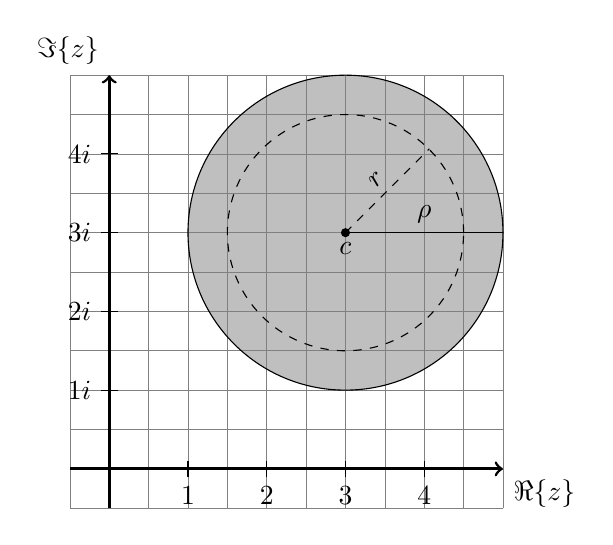
\begin{tikzpicture}
   % coords
   \coordinate (OR) at (0, 0);
   \coordinate (LX) at (-0.5, 0);
   \coordinate (RX) at (5, 0);
   \coordinate (TY) at (0, 5);
   \coordinate (BY) at (0, -0.5);

   % debugging grid
   \coordinate (BL) at (-0.5, -0.5);
   \coordinate (TR) at (5, 5);
   \draw[step=0.5cm, gray, very thin] (BL) grid (TR);

   % coordinate system
   \draw[->][line width=1.00pt] (LX) -- (RX) node[anchor=north west] {\(\Re\{z\}\)};
   \draw[->][line width=1.00pt] (BY) -- (TY) node[anchor=south east] {\(\Im\{z\}\)};
   \foreach \n in {1,2,...,4}{%
      \draw (\n,-3pt) node [below] {$\n$} -- (\n,3pt);
      \draw (-3pt,\n) node [left] {$\n i$} -- (3pt,\n);
   }

   \coordinate (c) at (3,3);
   \path[fill=gray, semitransparent] (c) circle (2);
   \draw[fill] (c) node[anchor=north]{\(c\)} circle [radius=0.05];
   \draw (c) circle (2);
   \draw (c) -- (5,3) node [midway, above, sloped, black] (TextNode) {\(\rho\)};

   \draw[dashed] (c) circle (1.5);
   \draw[dashed] (c) -- (4.065, 4.065) node [midway, above, sloped, black] (TextNode) {\(r\)};
\end{tikzpicture}

% \end{center}

\begin{theorem}[Power Series Convergence]\label{thm:conv_radius}
   Let \(\rho\) be the radius of convergence for \(\sum a_n z^n\).
   \[\forall z \in \mathbb{C}: \lvert z\rvert < \rho \implies \sum a_n z^n~\text{absolute convergent}\]
   \[\forall z \in \mathbb{C}: \lvert z\rvert > \rho \implies \sum a_n z^n~\text{divergent}\]
\end{theorem}
\begin{remark}
   For \(\lvert z\rvert = \rho\) we have to check for convergence seperately, i.e. we have to check if the series converges for \(z = \rho\) and \(z = -\rho\).
\end{remark}
\begin{example}
   For \(a_n := 1 \implies \sum_{n=0}^\infty z^n\) is \(\rho = 1\).
   The series converges to 0 for all \(|z| < 1\) and diverges for \(|z| \geq 1\).
\end{example}
\begin{example}
   For \(a_n := \frac{1}{n} \implies \sum_{n=0}^\infty \frac{1}{n} z^n\) is \(\rho = 1\).
   The series converges for \(|z| < 1\) and diverges for \(z = 1\).
   For \(z = -1\) is it the alternating harmonic series and converges.
\end{example}

\begin{proposition}[Important Power Series]
   The following are important examples of power series
   \begin{enumerate}[label=\roman*, align=Center]
      \item \(\forall z \in \mathbb{C}\)
         \[\sum_{n=0}^\infty \frac{1}{n!} z^n~\text{is absolute convergent}\]
      \item \(\forall z \in \mathbb{C}: \lvert z\rvert < 1\)
         \[\sum_{n=0}^\infty z^n~\text{is absolute convergent}\]
      \item Let \(z = 0\)
         \[\sum_{n=0}^\infty n! \cdot z^n~\text{is convergent}\]
      \item Let \(m \in \mathbb{Z}\) and \(\lvert z\rvert < 1\)
         \[\sum_{n=0}^\infty n^m \cdot z^n~\text{is convergent}\]
   \end{enumerate}
\end{proposition}

\begin{proposition}\label{pro:conv_rad_ratio_test}
   Let \(\rho\) be the radius of convergence of \(\sum a_n z^n\).
   \[\rho = \lim_{n \to \infty} \frac{\lvert a_n\rvert}{\lvert a_{n+1}\rvert}\]
\end{proposition}
\begin{remark}
   This proposition states that \(\rho\) can be calculated with the ratio test (\ref{pro:ratio_test}).
\end{remark}

\begin{theorem}
   Let \(\alpha \in \mathbb{C}\), \(\sum a_n z^n\) and \(\sum b_n z^n\) with radius of convergence \(\rho_a\) respectively \(\rho_b\).
   \begin{enumerate}[label=\roman*, align=Center]
      \item \(\forall z \in \mathbb{C}: \lvert z\rvert < \rho_a\)
         \[\sum \alpha \cdot a_n z^n = \alpha \cdot \sum a_n z^n\]
      \item \(\forall z \in \mathbb{C}: \lvert z\rvert < \min\{\rho_a, \rho_b\}\)
         \[\sum a_n z^n + \sum b_n z^n = \sum (a_n + b_n)z^n\]
      \item \(\forall \lvert z\rvert < \min\{\rho_a, \rho_b\}:\)
         \[\sum a_n z^n \cdot \sum b_n z^n = \sum_{n=0}^\infty\left(\sum_{k=0}^\infty a_k \cdot b_{n-k}\right)z^n\]
   \end{enumerate}
\end{theorem}

\subsection{Elementary Functions}
An \emph{elementary function} is a function of a single variable composed of particular simple functions.
They are typically defined as a sum, product, and/or composition of finitely many polynomials, rational functions, trigonometric and exponential functions, and their inverse functions.

\subsubsection{Exponential Function}
\begin{definition}[Exponential Function]
   Given \(z \in \mathbb{Z}\) we define \(\exp: \mathbb{C} \to \mathbb{C}\) by
   \[\exp(z) := \sum_{n = 0}^\infty \frac{z^n}{n!}\]
\end{definition}

\begin{proposition}[Properties]
   Let \(x, y, z \in \mathbb{C}\)
   \begin{enumerate}[label=\roman*, align=Center]
      \item The series has radius of convergence \(\rho = \infty\)
      \item \(\exp\) is continuous
      \item \(\exp(\alpha z) = \exp(z)^\alpha\)
      \item \(\exp(x + y) = \exp(x) \cdot \exp(y)\)
      \item \(\exp(-z) = \frac{1}{\exp(z)}\)
   \end{enumerate}
\end{proposition}

\begin{definition}[Eulers Number]
   \[e := \exp(1) = \sum_{n=0}^\infty \frac{1}{n!}\]
\end{definition}
\begin{remark}[Notation]
   From above we have \(e^z := \exp(z)\).
\end{remark}

Let \(z \in \mathbb{C}\), from above we see that
\[\exp(z) = \exp(x + iy) = \exp(x) \cdot \exp(iy)\]
which means that the complex \(\exp\) function is characterized by two parts
\[\exp: \mathbb{R} \to \mathbb{R} \qquad\text{and}\qquad \exp: i\mathbb{R} \to \mathbb{R}\]
We define the \emph{imaginary exponential function} \(\ixp: \mathbb{R} \to \mathbb{R}\) through \(\ixp(x) := \exp(ix)\).

\subsubsection{Logarithm}
\begin{proposition}
   We regard \(\exp: \mathbb{R} \to \mathbb{R}\), then
   \begin{enumerate}[label=\roman*, align=Center]
      \item \(\exp\) is strictly increasing
      \item \(\im(\exp) = \mathbb{R}_{>0}\)
      \item \(\forall n \in \mathbb{N}: \lim_{x \to \infty} \frac{\exp(x)}{x^n} = \infty\)
      \item \(\lim_{x \to -\infty} \exp(x) = 0\)
   \end{enumerate}
\end{proposition}
\begin{remark}[Intuition]
   We would split (ii) into the following observations:
   \[\forall x < 0: \exp(x) \in (0; 1) \qquad \forall x > 0: \exp(x) \in (1; \infty) \qquad \exp(0) = 1\]
   Point (iii) means that \(\exp\) grows faster than any other power.
\end{remark}

\begin{definition}[Logarithm]
   The inverse of \(\exp: \mathbb{R} \to \mathbb{R}_{>0}\) is
   \[\ln(x): \mathbb{R}_{>0} \to \mathbb{R} \qquad\text{where}\qquad \ln(x) = y \iff \exp(y) = x\]
\end{definition}

\begin{proposition}[Properties]
   Let \(x, y \in (0; \infty)\)
   \begin{enumerate}[label=\roman*, align=Center]
      \item \(\ln\) is continuous
      \item \(\ln\) is strictly increasing
      \item \(\lim_{x \to \infty} \ln(x) = \infty\)
      \item \(\lim_{x \to 0} \ln(x) = -\infty\)
      \item \(\ln(x^\alpha) = \alpha \cdot \ln(x)\)
      \item \(\ln(x \cdot y) = \ln(x) + \ln(y)\)
      \item \(\ln\left(\frac{x}{y}\right) = \ln(x) - \ln(y)\)
   \end{enumerate}
\end{proposition}
\begin{remark}
   From above we also have that \(\ln(1) = 0\).
\end{remark}

\subsubsection{Real Exponents}
Now that we have that \(x = \exp\big(\ln(x)\big)\) we can define \(x^r\) with \(r \in \mathbb{R}\).
First we need to check if everything remains the same as with whole exponents, so let \(n \in \mathbb{N}\) and \(x > 0\), then
\[x^n = \Big(\exp\big(\ln(x)\big)\Big)^n = \left(e^{\ln(x)}\right)^n = \exp\big(n \cdot \ln(x)\big)\]
\[x^{-n} = \frac{1}{x^n} = \frac{1}{\exp\big(n \cdot \ln(x)\big)} = \frac{1}{e^{n \cdot \ln(x)}} = e^{-n \cdot \ln(x)} = \exp\big(-n \cdot \ln(x)\big)\]
\[\sqrt[n]{x} = x^{\frac{1}{n}} = \Big(\exp\big(\ln(x)\big)\Big)^\frac{1}{n} = \exp\left(\frac{1}{n} \ln(x)\right)\]
and for \(p \in \mathbb{Z}\), \(q \in \mathbb{N}_{>0}\)
\[x^\frac{p}{q} = \Big(\exp\big(\ln(x)\big)\Big)^\frac{p}{q} = \exp\left(\frac{p}{q} \ln(x)\right)\]

\begin{definition}[Real Exponents]\label{def:real_exponents}
   Given \(x > 0\) and \(r \in \mathbb{R}\)
   \[x^r := \exp\big(r \cdot \ln(x)\big)\]
\end{definition}

\begin{proposition}[Calculation Rules]
   Let \(x, y \in \mathbb{R}_{>0}\) and \(r, s \in \mathbb{R}\), then
   \begin{enumerate}[label=\roman*, align=Center]
      \item \(x^r \cdot x^s = x^{r + s}\)
      \item \(\frac{x^r}{x^s} = x^{r-s}\)
      \item \(x^r \cdot y^r = (x \cdot y)^r\)
      \item \((x^r)^s = x^{r \cdot s}\)
      \item \(\ln(x^r) = r \cdot \ln(x)\)
   \end{enumerate}
\end{proposition}

\begin{proposition}
   Let \(r \in \mathbb{R}_{>0}\) then
   \[\lim_{x \to \infty} \left(x^{-r} \cdot \ln(x)\right) = 0 \qquad\text{and}\qquad \lim_{x \to 0} \left(x^r \cdot \ln(x)\right) = 0\]
\end{proposition}
\begin{remark}
   This proposition states that \(\ln\) is damped by \(\frac{1}{x^n}\).
\end{remark}

\subsubsection{Trigonometric Functions}
\begin{definition}[Cosine]
   Given \(z \in \mathbb{C}\) we define \(\cos: \mathbb{C} \to \mathbb{C}\) by
   \[\cos(z) := \sum_{n=0}^\infty (-1)^n \frac{z^{2n}}{(2n)!}\]
\end{definition}

\begin{definition}[Sine]
   Given \(z \in \mathbb{C}\) we define \(\sin: \mathbb{C} \to \mathbb{C}\) by
   \[\sin(z) := \sum_{n=0}^\infty (-1)^n \frac{z^{2n + 1}}{(2n+1)!}\]
\end{definition}

\begin{proposition}[Properties]
   Let \(z, w \in \mathbb{C}\), then
   \begin{enumerate}[label=\roman*, align=Center]
      \item Both series have radius of convergence \(\rho = \infty\)
      \item \(\cos\) and \(\sin\) are continuous
      \item \(\cos(-z) = \cos(z)\)
      \item \(\sin(-z) = -\sin(z)\)
      \item \(\cos(z \pm w) = \cos(z) \cdot \cos(w) \mp \sin(z) \cdot \sin(w)\)
      \item \(\sin(z \pm w) = \sin(z) \cdot \cos(w) \pm \cos(z) \cdot \sin(w)\)
      \item \(\sin(z) - \sin(w) = 2 \cos\left(\frac{z+w}{2}\right) \cdot \sin\left(\frac{z-w}{2}\right)\)
      \item \(\cos(z) - \cos(w) = -2 \sin\left(\frac{z+w}{2}\right) \cdot \sin\left(\frac{z-w}{2}\right)\)
      \item \(\cos^2(z) + \sin^2(z) = 1\)
   \end{enumerate}
\end{proposition}

\subsubsection{Connecting Exponential and Trigonometric}
Recall that \(\ixp(x) := \exp(ix)\).

\begin{proposition}
   Let \(x \in \mathbb{R}\) and \(z \in \mathbb{C}\), then
   \begin{enumerate}[label=\roman*, align=Center]
      \item \(\cos(x) = \Re\big(\exp(ix)\big)\)
      \item \(\sin(x) = \Im\big(\exp(ix)\big)\)
      \item \(\exp(ix) = \cos(x) + i \cdot \sin(x)\)
      \item \[\cos(z) = \frac{\exp(iz) + \exp(-iz)}{2}\]
      \item \[\sin(z) = \frac{\exp(iz) - \exp(-iz)}{2i}\]
   \end{enumerate}
\end{proposition}

\begin{theorem}[Unit Circle]
   \(\im(\ixp) = S^1 := \{z \in \mathbb{C} \mid \lvert z\rvert = 1\}\)
\end{theorem}
\begin{center}
   \begin{tikzpicture}[line cap=round,line join=round,>=triangle 45,x=1cm,y=1cm]
   \begin{axis}[
   x=5cm,y=5cm,
   axis lines=middle,
   ymajorgrids=true,
   xmajorgrids=true,
   xmin=-1.1, xmax=1.1,
   ymin=-1.1, ymax=1.1,
   xtick={-1,-0.8,...,1},
   ytick={-1,-0.8,...,1},]

   \draw [line width=2pt,color=black] (0,0) circle (5cm);

   \draw [line width=2pt, color=black] (0,0)-- (0.6,0.8);

   \draw [line width=1pt, dashed]  (0.6,0)-- (0.6,0.8);
   \draw [line width=1pt, dashed] (0,0.8)-- (0.6,0.8);

   \draw [line width=2pt,color=red] (0,0)-- (0.6,0);
   \draw [line width=2pt,color=blue] (0,0)-- (0,0.8);

   \draw [fill=grey] (0.6,0.8) circle (2.5pt);
   \draw (0.67, 0.87 ) node {\(e^{it}\)};
   \draw (-0.6, 1) node {\(\{z \in \mathbb{C} \mid |z| = 1\}\)};

   \draw (0.3, 0.05) node {\(\cos(t)\)};
   \draw (0.12, 0.4) node {\(\sin(t)\)};
   \end{axis}
\end{tikzpicture}

\end{center}

\begin{theorem}
   The set
   \[M := \{x \in (0; \infty) \mid \ixp(x) = 1\}\]
   has a positive minimum
   \[\pi := \frac{1}{2} \min(M)\]
\end{theorem}

\begin{definition}[Periodic Function]
   \(f: \mathbb{K} \to \mathbb{K}\) is \(p\)-periodic iff
   \[\forall x \in \mathbb{K}: f(x + p) = f(x)\]
\end{definition}

\begin{theorem}
   Let \(z \in \mathbb{C}\) and \(k \in \mathbb{Z}\), then
   \[\exp(z) = 1 \iff z = 2 \pi i \cdot k\]
   \[\exp(z) = -1 \iff z = (2k + 1)\pi i\]
\end{theorem}
\begin{remark}
   It follows that for \(k \in \mathbb{Z}\) holds \(\exp(z) = \exp(z + 2k\pi i)\) i.e. \(\exp\) is \(2\pi i\)-periodic.
\end{remark}

\begin{theorem}
   For \(x \in \mathbb{R}\) is \(\ixp: [x; x + 2\pi) \to S^1\) bijective.
\end{theorem}

\begin{proposition}[Properties]
   Let \(k \in \mathbb{Z}\) and \(z \in \mathbb{C}\), then
   \begin{enumerate}[label=\roman*, align=Center]
      \item \(\cos(z) = \cos(z + 2k\pi)\)
      \item \(\cos(k\pi) = (-1)^k\)
      \item \(\sin(z) = \sin(z + 2k\pi)\)
      \item \(\sin\left((2k+1)\frac{\pi}{2}\right) = (-1)^k\)
      \item \(\cos(z) = 0 \iff z = \frac{\pi}{2} + k\pi\)
      \item \(\sin(z) = 0 \iff z = k\pi\)
      \item \(\forall x \in (0; \pi): \sin(x) > 0\)
      \item \(\forall x \in \left(0; \frac{\pi}{2}\right): \cos(x) > 0\)
      \item \(\sin\) is strictly increasing on \(\left[0; \frac{\pi}{2}\right]\)
      \item \(\sin(z + \pi) = -\sin(z)\)
      \item \(\cos(z + \pi) = -\cos(z)\)
      \item \(\sin\left(\frac{\pi}{2} - z\right) = \cos(z)\)
      \item \(\cos\left(\frac{\pi}{2} - z\right) = \sin(z)\)
      \item \(\im(\cos) = \im(\sin) = [-1;1]\)
   \end{enumerate}
\end{proposition}
\begin{remark}
   The following table displays common values of the trigonometric functions.
   \begin{center}
      \renewcommand\arraystretch{1.3}
      \begin{tabular}{c|c|c|c|c|c}
              & \(0^\circ\) & \(30^\circ\) & \(45^\circ\) & \(60^\circ\) & \(90^\circ = \frac{\pi}{2}\)\\
         \hline
         \(\sin\) & \(\frac{\sqrt{0}}{2}\) & \(\frac{\sqrt{1}}{2}\) & \(\frac{\sqrt{2}}{2}\) & \(\frac{\sqrt{3}}{2}\) & \(\frac{\sqrt{4}}{2}\)\\
         \hline
         \(\cos\) & \(\frac{\sqrt{4}}{2}\) & \(\frac{\sqrt{3}}{2}\) & \(\frac{\sqrt{2}}{2}\) & \(\frac{\sqrt{1}}{2}\) & \(\frac{\sqrt{0}}{2}\)\\
      \end{tabular}
   \end{center}
\end{remark}

\begin{theorem}
   For \(x \in \mathbb{R}\) is \(\exp: \mathbb{R} + i[x; x + 2\pi) \to \mathbb{C}\setminus\{0\}\) bijective.
\end{theorem}

\begin{theorem}[Polar Coordinates]
   For any \(z \in \mathbb{C}\setminus\{0\}\),
   \[\exists! \theta \in [0; 2\pi): z = \lvert z\rvert \cdot \exp(i \theta)\]
\end{theorem}
We call \(\theta\) the \emph{argument} of \(z\), denoted \(\argu(z) := \theta\).
With this we can derive \emph{polar coordinates} of any complex number \(z\)
\[z = x + iy = r \cdot \exp(i \theta) \qquad\text{where}~r := |z| = \sqrt{x^2 + y^2}\]
The values \(x\) and \(y\) are called the \emph{Cartesian coordinates} of \(z\), while \(r\) and \(\theta\) are its \emph{polar coordinates}.
Now note that
\[z = x + iy = \lvert z\rvert \cdot \exp(i \theta) = \lvert z \rvert \cdot \big(\cos(\theta) + i\sin(\theta)\big) = \lvert z\rvert\cos(\theta) + i\lvert z\rvert\sin(\theta)\]
hence we have
\[\cos(\theta) = \frac{\Re(z)}{\lvert z\rvert} \qquad\text{and}\qquad \sin(\theta) = \frac{\Im(z)}{\lvert z\rvert}\]
\begin{example}
   Let \(z := -\sqrt{3} + i3\), we compute its polar coordinates.

   First we compute \(\lvert z\rvert = \sqrt{(-\sqrt{3})^2 + 3^2} = \sqrt{12}\).
   Then we solve
   hence
   \[-\sqrt{3} + i3 = \sqrt{12}\cos(\theta) + i\sqrt{12}\sin(\theta) \implies \begin{cases}
         -\sqrt{3} = \sqrt{12}\cos(\theta) \implies \cos(\theta) = -\frac{\sqrt{3}}{\sqrt{12}} = -\frac{1}{2}\\
         3 = \sqrt{12}\sin(\theta) \implies \sin(\theta) = \frac{3}{\sqrt{12}} = \frac{\sqrt{3}}{2}
   \end{cases}\]
   Now we lookup the values on the unit circle and get that \(\theta = \frac{2\pi}{3}\).
\end{example}

% TODO: make better drawing
% \begin{center}
%    \begin{tikzpicture}[line cap=round,line join=round,>=triangle 45,x=1cm,y=1cm]
   \begin{axis}[
   x=1cm,y=1cm,
   axis lines=middle,
   ymajorgrids=true,
   xmajorgrids=true,
   xmin=-3.6423644972783227,
   xmax=9.836484290540891,
   ymin=-2.466863579845977,
   ymax=5.846571116588563,
   xtick={-3,-2,...,9},
   ytick={-2,-1,...,5},]
      \draw [shift={(0,0)},line width=2pt,fill=black,fill opacity=0.10000000149011612] (0,0) -- (0:0.33253738785738196) arc (0:30.96375653207352:0.33253738785738196) -- cycle;
      \draw [line width=1.2pt,dashed] (5,3)-- (5,0);
      \draw [line width=1.2pt,dashed] (5,3)-- (0,3);
      \draw [line width=2pt,color=grey] (0,0)-- (5,3);
      \draw [line width=2pt,color=blue] (0,0)-- (0,3);
      \draw [line width=2pt,color=red] (0,0)-- (5,0);
      \draw [fill=blue] (5,3) circle (2.5pt);
      \draw[color=blue] (6.466772093586088,3.236152621908117) node {\(z = x + iy = |z| * \exp(i\theta)\)};
      \draw[color=grey] (2.7201841903929185,1.4847890458592405) node {|z|};
      \draw[color=black] (0.6695369652723964,0.1878932332154525) node {\(\theta\)};
      \draw[color=blue] (-0.18397566356155054,1.5956348418117012) node {\(iy\)};
      \draw[color=red] (2.5428309168689816,-0.044882938284714596) node {\(x\)};
   \end{axis}
\end{tikzpicture}

% \end{center}

\begin{theorem}[Complex nth-Root]
   For \(x \in \mathbb{C}\) has \(z^n = x\) \(n\) distinct solutions
   \[z_k = \lvert x\rvert^\frac{1}{n} \exp\left(\frac{i(\argu(x) + 2\pi k)}{n}\right)\]
\end{theorem}
\begin{example}
   We want to find the 6th roots of \(x := 4 + i4\sqrt{3}\).

   So first we compute
   \[\lvert x\rvert = \sqrt{4^2 +4^2\cdot 3} = \sqrt{64} = 8 \rightsquigarrow \cos(\theta)=\frac{4}{8} = \frac{1}{2} \quad \sin(\theta) = \frac{4\sqrt{3}}{8} = \frac{\sqrt{3}}{2}\]
   where we get \(\theta = \frac{\pi}{3} = \argu(x)\)
   So we can compute our 6 solutions with the theorem above
   \[z_k = \sqrt[6]{8} \cdot \exp\left(\frac{i(\frac{\pi}{3} + 2\pi k)}{6}\right) = \sqrt[6]{8} \left(\cos\left(\frac{\pi}{18} + \frac{\pi}{3} k\right) + i \sin\left(\frac{\pi}{18} + \frac{\pi}{3}k\right)\right)\]
   hence we get
   \[z_0 = \sqrt[6]{8}\left(\cos\left(\frac{\pi}{18}\right) + i\sin\left(\frac{\pi}{18}\right)\right)\]
   \[z_1 = \sqrt[6]{8}\left(\cos\left(\frac{7\pi}{18}\right) + i\sin\left(\frac{7\pi}{18}\right)\right)\]
   \[z_2 = \sqrt[6]{8}\left(\cos\left(\frac{13\pi}{18}\right) + i\sin\left(\frac{13\pi}{18}\right)\right)\]
   \[z_3 = \sqrt[6]{8}\left(\cos\left(\frac{19\pi}{18}\right) + i\sin\left(\frac{19\pi}{18}\right)\right)\]
   \[z_4 = \sqrt[6]{8}\left(\cos\left(\frac{25\pi}{18}\right) + i\sin\left(\frac{25\pi}{18}\right)\right)\]
   \[z_5 = \sqrt[6]{8}\left(\cos\left(\frac{31\pi}{18}\right) + i\sin\left(\frac{31\pi}{18}\right)\right)\]
\end{example}

\newpage

\section{Continuity}
A rigorous definition of continuity of real functions is usually given in terms of the idea of a limit of those functions.
So far we only looked at limits of sequences, so now we want to regard the limit of functions.

\subsection{Function Limits}\label{ssec:function_limits}
\begin{definition}[Function Limit]\label{def:func_limit}
   Given \(f: D \to \mathbb{R}\) and \(x_0 \in D\),
   \[\lim_{x \to x_0}\big(f(x)\big) = L :\iff \forall \varepsilon > 0~\exists \delta > 0: (\forall x \in D: \lvert x - x_0 \rvert < \delta \implies \lvert f(x) - L\rvert < \varepsilon\]
\end{definition}
\begin{remark}[Intuition]
   Note that we can rewrite the condition above as
   \[\forall x \in (x_0 - \delta; x_0 + \delta): f(x) \in \big(L - \varepsilon; L + \varepsilon\big)\]
   \begin{center}
      \begin{tikzpicture}[line cap=round,line join=round,>=triangle 45,x=1cm,y=1cm]
   \begin{axis}[
   ticks=none,
   x=2cm, y=2cm,
   axis lines=middle,
   ymajorgrids=true,
   xmajorgrids=true,
   xmin=-0.4, xmax=6.1,
   ymin=-0.4, ymax=3.1]
      \fill[line width=2pt,color=gray,fill=gray,fill opacity=0.1] (0,2.2) -- (8,2.2) -- (8,1) -- (0,1) -- cycle;
      \draw[line width=2pt,color=blue,smooth,samples=100,domain=-0.3:7] plot(\x,{ln((\x)+1)});

      \draw [line width=1pt,dashed] (0,1.6079667094364514) -- (4.000000075430033,1.6094379275201067);
      \draw [line width=1pt,dashed] (4.000000075430033,1.6094379275201067)-- (4,0);
      \draw [line width=1pt] (3,0) -- (2.9996517855796725,1.3862073037254237);
      \draw [line width=1pt] (5,0) -- (5.000842962216623,1.7918999530625097);
      \draw [line width=1pt] (0,2.2) -- (8,2.2);
      \draw [line width=1pt] (8,1) -- (0,1);

      \draw [line width=4pt,color=orange] (2.9996517855796725,1.3862073037254237)-- (3.199034292788041,1.4348545685627394)-- (3.399609048748734,1.4815156844194872)-- (3.5985123484097543,1.5257328486695583)-- (3.799087104370447,1.5684257132365922)-- (4.000000075430033,1.6094379275201067)-- (4.200236616291833,1.6487041276851904)-- (4.402482828552198,1.6868586309676052)-- (4.6013861282132185,1.7230140900075834)-- (4.8002894278742385,1.7579078176649696)-- (5.000842962216623,1.7918999530625097);

      \draw [fill=blue] (0,2.2) circle (2.5pt);
      \draw (0.39, 2.33) node {\(L + \varepsilon\)};
      \draw [fill=blue] (0,1.6079667094364514) circle (2.5pt);
      \draw (0.29, 1.7408231122516713) node {\(L\)};
      \draw [fill=blue] (0,1) circle (2.5pt);
      \draw (0.39, 1.13) node {\(L - \varepsilon\)};

      \draw [fill=blue] (4.000000075430033,1.6094379275201067) circle (2.5pt);

      \draw [fill=blue] (5,0) circle (2.5pt);
      \draw (5, -0.15) node {\(x_0 + \delta\)};
      \draw [fill=blue] (4,0) circle (2.5pt);
      \draw (4, -0.15) node {\(x_0\)};
      \draw [fill=blue] (3,0) circle (2.5pt);
      \draw (3, -0.15) node {\(x_0 - \delta\)};
   \end{axis}
\end{tikzpicture}

   \end{center}
\end{remark}
Now we see that the concept of the limit of a function is connected to the concept of the limit of sequences.
\begin{proposition}[Function Limit = Sequence Limit]
   Let \(f: D \to \mathbb{R}\) and \(x_0 \in X\),
   \[\lim_{x \to x_0}\big(f(x)\big) = L \iff \forall x_n \in \big(D\setminus\{x_0\}\big)^\mathbb{N}: \left(\lim_{n \to \infty}(x_n) = x_0 \implies  \lim_{n \to \infty}\big(f(x_n)\big) = L\right)\]
\end{proposition}
\begin{remark}[Intuition]
   We regard all sequences \(x_n\) in the domain of \(f\) which converge to the input \(x_0\).
   Then we take each sequence, use it as inputs for \(f\) and create a sequence of function values.
   If all those sequences of function values converge to \(L\), we say \(L\) is the limit of \(f\) as \(x \to x_0\).
\end{remark}

\subsubsection{Computing Function Limits}
As the limit of sequences and functions are equivalent we can derive calculation rules for function limits from \cref{pro:seq_limit_rules}.
\begin{proposition}[Function Limit Rules]
   Let \(f: I \to \mathbb{R}\), \(g: I \to \mathbb{R}\) and \(c \in \mathbb{R}\), then

   \begin{enumerate}[label=\roman*, align=Center]
      \item \[\lim_{x \to x_0}\big(f(x) \pm g(x)\big) = \lim_{x \to x_0}\big(f(x)\big) \pm \lim_{x \to x_0}\big(g(x)\big)\]
      \item \[\lim_{x \to x_0}\big(c \cdot f(x)\big) = c \cdot \lim_{x \to x_0}\big(f(x)\big)\]
      \item \[\lim_{x \to x_0}\big(f(x) \cdot g(x)\big) = \lim_{x \to x_0}\big(f(x)\big) \cdot \lim_{x \to x_0}\big(g(x)\big)\]
      \item \[\lim_{x \to x_0}\left(\frac{f(x)}{g(x)}\right) = \frac{\lim_{x \to x_0}\big(f(x)\big)}{\lim_{x \to x_0}\big(g(x)\big)}\]
   \end{enumerate}
\end{proposition}

\paragraph{The Root-Trick} is a usefull method to determine limits which contain \(\sqrt{x}\).
\begin{example}
   We want to find \(\lim_{x \to \infty}\big(f(x)\big)\) where \(f(x) := \sqrt{x^2 + x} - x\).
\begin{equation*}
   \begin{split}
      \lim_{x \to \infty} \left(\sqrt{x^2 + x} - x\right) & = \lim_{x \to \infty} \left(\left(\sqrt{x^2 + x} - x\right) \frac{\left(\sqrt{x^2 + x} + x\right)}{\left(\sqrt{x^2 + x} + x\right)}\right) = \lim_{x \to \infty} \left(\frac{x^2 + x - x^2}{\sqrt{x^2 + x} + x}\right) =\\
                                                          & = \lim_{x \to \infty} \left(\frac{x}{\sqrt{x^2 + x} + x}\right) = \lim_{x \to \infty}\left(\frac{x}{x \left(\frac{\sqrt{x^2 + x}}{x} + 1\right)}\right) = \frac{1}{\lim_{x \to \infty}\left(\frac{\sqrt{x^2 + x}}{x} + 1\right)} =\\
                                                          & = \frac{1}{\lim_{x \to \infty}\left(\sqrt{\frac{x^2 + x}{x^2}}\right) + 1} = \frac{1}{\sqrt{\lim_{x \to \infty}\left(\frac{x^2 \left(1 + \frac{1}{x}\right)}{x^2}\right)} + 1} = \frac{1}{\sqrt{\lim_{x \to \infty}\left(1 + \frac{1}{x}\right)} + 1} =\\
                                                          & = \frac{1}{\sqrt{1} + 1} = \frac{1}{2}
   \end{split}
\end{equation*}
\end{example}

\paragraph{The Fundamental Limit \(e\)} is given by
\[\lim_{x \to \infty} \left(1 + \frac{1}{x}\right)^x = e \qquad\text{and}\qquad \lim_{x \to 0} (1 + x)^{\frac{1}{x}} = e\]
From this follows (not trivially) a neat trick:
\[\lim_{x \to x_0} \left(1 + \frac{1}{\ast}\right)^* = e\]
where \(\ast\) is some term in \(x\) with \(\ast \xrightarrow{x \to x_0} \infty\).
Equivalently we have
\[\lim_{x \to x_0} (1 + \ast)^{\frac{1}{\ast}} = e\]
where \(\ast \xrightarrow{x \to x_0} 0\).
\begin{example}
   We want to find \(\lim_{x \to \infty}\big(f(x)\big)\) where \(f(x) := \left(1 - \frac{3}{x}\right)^{2x}\).
   \[\lim_{x \to \infty} \left(1 - \frac{3}{x}\right)^{2x} = \lim_{x \to \infty} \left(\left(1 + \frac{1}{-\frac{x}{3}}\right)^{-\frac{x}{3}}\right)^{-\frac{3}{x} \cdot 2x} = \lim_{x \to \infty}\Big(e^{-\frac{6x}{x}}\Big) = e^{-6}\]
\end{example}

\paragraph{The Fundamental Limit \(\sin(x)\)} is given by
\[\lim_{x \to 0}\left(\frac{\sin(x)}{x}\right) = 1\]
From this follows a neat trick:
\[\lim_{x \to x_0} \frac{\sin(\ast)}{\ast} = 1\]
where \(\ast\) is some term in \(x\) with \(\ast \xrightarrow{x \to x_0} 0\).
\begin{example}
   We want to find \(\lim_{x \to 1} \frac{\sin(1-x^2)}{1-x}\)
   \[\lim_{x \to 1} \frac{\sin(1-x^2)}{1-x} = \lim_{x \to 1}\frac{\sin(1-x^2)}{1-x^2} \cdot \frac{1-x^2}{1-x} = 1 \cdot \lim_{x \to 1} \frac{(1-x)(1+x)}{1-x} = \lim_{x \to 1} 1 + x = 2\]
\end{example}

\paragraph{The \(e^{\log}\) - Trick} derived from \cref{def:real_exponents}, is a usefull method to determine limits \(\lim_{x \to x_0} f(x)^{g(x)}\).
The main idea is to rewrite
\[f(x)^{g(x)} = \exp\Big(\log\big(f(x)^{g(x)}\big)\Big) = \exp\Big(g(x) \cdot \log\big(f(x)\big)\Big)\]
as \(\exp\) is continuous, we can pull the limit into the argument.
\begin{equation*}
   \begin{split}
      \lim_{x \to x_0} f(x)^{g(x)} &= \lim_{x \to x_0} e^{\log(f(x)^{g(x)})} = \lim_{x \to x_0} e^{g(x) \cdot \log(f(x))} \overset{e~\text{cont.}}{=} \exp\left(\lim_{x \to x_0} \Big(g(x) \cdot log\big(f(x)\big)\Big)\right) = \\
                                   & = \exp\left(\lim_{x \to x_0}g(x) \cdot \lim_{x \to x_0}\Big(\log\big(f(x)\big)\Big)\right) \overset{\ln~\text{cont.}}{=} \exp\left(\lim_{x \to x_0}g(x) \cdot \log\left(\lim_{x \to x_0}f(x)\right)\right)
   \end{split}
\end{equation*}
% TODO
\begin{example}
\end{example}

\subsubsection{One-Sided Limits}
Another intuitive viewpoint to see how function limits and continuity are connected is the following.
\begin{definition}[One-Sided Limit]\label{def:one-sided_limit}
   Given \(x_0 \in \overline{\mathbb{R}}\) and \(f: [a;b] \to \mathbb{R}\),
   \[\lim_{x \uparrow x_0}\big(f(x)\big) := \lim_{x \to x_0}\big(f|_{D \cap (-\infty; x_0)}\big)\]
   \[\lim_{x \downarrow x_0}\big(f(x)\big) := \lim_{x \to x_0}\big(f|_{D \cap (x_0; \infty)}\big)\]
\end{definition}
\begin{remark}[Terminology]
   We call \(\lim_{x \uparrow x_0} f(x)\) a \emph{left-handed} and \(\lim_{x \downarrow x_0} f(x)\) a \emph{right-handed} limit.
\end{remark}
\begin{remark}[Notation]
   There are many equivalent ways of denoting left- and right-handed limits
   \[\lim_{x \downarrow x_0}\big(f(x)\big) \qquad \lim_{x \to x_0^+}\big(f(x)\big) \qquad \lim_{x \searrow x_0}\big(f(x)\big)\]
   \[\lim_{x \uparrow x_0}\big(f(x)\big) \qquad \lim_{x \to x_0^-}\big(f(x)\big) \qquad \lim_{x \nearrow x_0}\big(f(x)\big)\]
\end{remark}
\begin{remark}
   From \cref{def:func_limit} we can equivalently write
   \[\lim_{x \uparrow x_0} f(x) = L \iff \forall \varepsilon~\exists \delta > 0: (x \in D: x_0- \delta < x < x_0 \implies |f(x) - L| < \varepsilon)\]
   \[\lim_{x \downarrow x_0} f(x) = L \iff \forall \varepsilon~\exists \delta > 0: (x \in D: x_0 < x < x_0 + \delta \implies |f(x) - L| < \varepsilon)\]
\end{remark}
\begin{example}
   We regard
   \[f(x) = \begin{cases}0 & x \leq 0\\ 1 & x > 0\end{cases}\]
   where we see that
   \[\lim_{x \uparrow 0} f(x) = 0 \qquad \lim_{x \downarrow 0} f(x) = 1\]
\end{example}
\begin{center}
   \begin{tikzpicture}[line cap=round,line join=round,>=triangle 45,x=1cm,y=1cm]
   \begin{axis}[
   x=4cm,y=4cm,
   axis lines=middle,
   ymajorgrids=true,
   xmajorgrids=true,
   xmin=-0.7,
   xmax=0.7,
   ymin=-0.1,
   ymax=1.1,
   xtick={-1,0,1},
   ytick={-1,0,1},]
   \draw[line width=2pt,color=blue] (-1.2292426079511276,0) -- (-1.2292426079511276,0);
   \draw[line width=2pt,color=blue] (-1.2292426079511276,0) -- (-1.2226596040846602,0);
   \draw[line width=2pt,color=blue] (-1.2226596040846602,0) -- (-1.2160766002181929,0);
   \draw[line width=2pt,color=blue] (-1.2160766002181929,0) -- (-1.2094935963517255,0);
   \draw[line width=2pt,color=blue] (-1.2094935963517255,0) -- (-1.2029105924852581,0);
   \draw[line width=2pt,color=blue] (-1.2029105924852581,0) -- (-1.1963275886187907,0);
   \draw[line width=2pt,color=blue] (-1.1963275886187907,0) -- (-1.1897445847523234,0);
   \draw[line width=2pt,color=blue] (-1.1897445847523234,0) -- (-1.183161580885856,0);
   \draw[line width=2pt,color=blue] (-1.183161580885856,0) -- (-1.1765785770193886,0);
   \draw[line width=2pt,color=blue] (-1.1765785770193886,0) -- (-1.1699955731529212,0);
   \draw[line width=2pt,color=blue] (-1.1699955731529212,0) -- (-1.1634125692864539,0);
   \draw[line width=2pt,color=blue] (-1.1634125692864539,0) -- (-1.1568295654199865,0);
   \draw[line width=2pt,color=blue] (-1.1568295654199865,0) -- (-1.1502465615535191,0);
   \draw[line width=2pt,color=blue] (-1.1502465615535191,0) -- (-1.1436635576870517,0);
   \draw[line width=2pt,color=blue] (-1.1436635576870517,0) -- (-1.1370805538205844,0);
   \draw[line width=2pt,color=blue] (-1.1370805538205844,0) -- (-1.130497549954117,0);
   \draw[line width=2pt,color=blue] (-1.130497549954117,0) -- (-1.1239145460876496,0);
   \draw[line width=2pt,color=blue] (-1.1239145460876496,0) -- (-1.1173315422211823,0);
   \draw[line width=2pt,color=blue] (-1.1173315422211823,0) -- (-1.1107485383547149,0);
   \draw[line width=2pt,color=blue] (-1.1107485383547149,0) -- (-1.1041655344882475,0);
   \draw[line width=2pt,color=blue] (-1.1041655344882475,0) -- (-1.0975825306217801,0);
   \draw[line width=2pt,color=blue] (-1.0975825306217801,0) -- (-1.0909995267553128,0);
   \draw[line width=2pt,color=blue] (-1.0909995267553128,0) -- (-1.0844165228888454,0);
   \draw[line width=2pt,color=blue] (-1.0844165228888454,0) -- (-1.077833519022378,0);
   \draw[line width=2pt,color=blue] (-1.077833519022378,0) -- (-1.0712505151559106,0);
   \draw[line width=2pt,color=blue] (-1.0712505151559106,0) -- (-1.0646675112894433,0);
   \draw[line width=2pt,color=blue] (-1.0646675112894433,0) -- (-1.0580845074229759,0);
   \draw[line width=2pt,color=blue] (-1.0580845074229759,0) -- (-1.0515015035565085,0);
   \draw[line width=2pt,color=blue] (-1.0515015035565085,0) -- (-1.0449184996900411,0);
   \draw[line width=2pt,color=blue] (-1.0449184996900411,0) -- (-1.0383354958235738,0);
   \draw[line width=2pt,color=blue] (-1.0383354958235738,0) -- (-1.0317524919571064,0);
   \draw[line width=2pt,color=blue] (-1.0317524919571064,0) -- (-1.025169488090639,0);
   \draw[line width=2pt,color=blue] (-1.025169488090639,0) -- (-1.0185864842241716,0);
   \draw[line width=2pt,color=blue] (-1.0185864842241716,0) -- (-1.0120034803577043,0);
   \draw[line width=2pt,color=blue] (-1.0120034803577043,0) -- (-1.005420476491237,0);
   \draw[line width=2pt,color=blue] (-1.005420476491237,0) -- (-0.9988374726247695,0);
   \draw[line width=2pt,color=blue] (-0.9988374726247695,0) -- (-0.9922544687583021,0);
   \draw[line width=2pt,color=blue] (-0.9922544687583021,0) -- (-0.9856714648918348,0);
   \draw[line width=2pt,color=blue] (-0.9856714648918348,0) -- (-0.9790884610253674,0);
   \draw[line width=2pt,color=blue] (-0.9790884610253674,0) -- (-0.9725054571589,0);
   \draw[line width=2pt,color=blue] (-0.9725054571589,0) -- (-0.9659224532924326,0);
   \draw[line width=2pt,color=blue] (-0.9659224532924326,0) -- (-0.9593394494259653,0);
   \draw[line width=2pt,color=blue] (-0.9593394494259653,0) -- (-0.9527564455594979,0);
   \draw[line width=2pt,color=blue] (-0.9527564455594979,0) -- (-0.9461734416930305,0);
   \draw[line width=2pt,color=blue] (-0.9461734416930305,0) -- (-0.9395904378265632,0);
   \draw[line width=2pt,color=blue] (-0.9395904378265632,0) -- (-0.9330074339600958,0);
   \draw[line width=2pt,color=blue] (-0.9330074339600958,0) -- (-0.9264244300936284,0);
   \draw[line width=2pt,color=blue] (-0.9264244300936284,0) -- (-0.919841426227161,0);
   \draw[line width=2pt,color=blue] (-0.919841426227161,0) -- (-0.9132584223606937,0);
   \draw[line width=2pt,color=blue] (-0.9132584223606937,0) -- (-0.9066754184942263,0);
   \draw[line width=2pt,color=blue] (-0.9066754184942263,0) -- (-0.9000924146277589,0);
   \draw[line width=2pt,color=blue] (-0.9000924146277589,0) -- (-0.8935094107612915,0);
   \draw[line width=2pt,color=blue] (-0.8935094107612915,0) -- (-0.8869264068948242,0);
   \draw[line width=2pt,color=blue] (-0.8869264068948242,0) -- (-0.8803434030283568,0);
   \draw[line width=2pt,color=blue] (-0.8803434030283568,0) -- (-0.8737603991618894,0);
   \draw[line width=2pt,color=blue] (-0.8737603991618894,0) -- (-0.867177395295422,0);
   \draw[line width=2pt,color=blue] (-0.867177395295422,0) -- (-0.8605943914289547,0);
   \draw[line width=2pt,color=blue] (-0.8605943914289547,0) -- (-0.8540113875624873,0);
   \draw[line width=2pt,color=blue] (-0.8540113875624873,0) -- (-0.8474283836960199,0);
   \draw[line width=2pt,color=blue] (-0.8474283836960199,0) -- (-0.8408453798295525,0);
   \draw[line width=2pt,color=blue] (-0.8408453798295525,0) -- (-0.8342623759630852,0);
   \draw[line width=2pt,color=blue] (-0.8342623759630852,0) -- (-0.8276793720966178,0);
   \draw[line width=2pt,color=blue] (-0.8276793720966178,0) -- (-0.8210963682301504,0);
   \draw[line width=2pt,color=blue] (-0.8210963682301504,0) -- (-0.814513364363683,0);
   \draw[line width=2pt,color=blue] (-0.814513364363683,0) -- (-0.8079303604972157,0);
   \draw[line width=2pt,color=blue] (-0.8079303604972157,0) -- (-0.8013473566307483,0);
   \draw[line width=2pt,color=blue] (-0.8013473566307483,0) -- (-0.7947643527642809,0);
   \draw[line width=2pt,color=blue] (-0.7947643527642809,0) -- (-0.7881813488978135,0);
   \draw[line width=2pt,color=blue] (-0.7881813488978135,0) -- (-0.7815983450313462,0);
   \draw[line width=2pt,color=blue] (-0.7815983450313462,0) -- (-0.7750153411648788,0);
   \draw[line width=2pt,color=blue] (-0.7750153411648788,0) -- (-0.7684323372984114,0);
   \draw[line width=2pt,color=blue] (-0.7684323372984114,0) -- (-0.761849333431944,0);
   \draw[line width=2pt,color=blue] (-0.761849333431944,0) -- (-0.7552663295654767,0);
   \draw[line width=2pt,color=blue] (-0.7552663295654767,0) -- (-0.7486833256990093,0);
   \draw[line width=2pt,color=blue] (-0.7486833256990093,0) -- (-0.7421003218325419,0);
   \draw[line width=2pt,color=blue] (-0.7421003218325419,0) -- (-0.7355173179660746,0);
   \draw[line width=2pt,color=blue] (-0.7355173179660746,0) -- (-0.7289343140996072,0);
   \draw[line width=2pt,color=blue] (-0.7289343140996072,0) -- (-0.7223513102331398,0);
   \draw[line width=2pt,color=blue] (-0.7223513102331398,0) -- (-0.7157683063666724,0);
   \draw[line width=2pt,color=blue] (-0.7157683063666724,0) -- (-0.7091853025002051,0);
   \draw[line width=2pt,color=blue] (-0.7091853025002051,0) -- (-0.7026022986337377,0);
   \draw[line width=2pt,color=blue] (-0.7026022986337377,0) -- (-0.6960192947672703,0);
   \draw[line width=2pt,color=blue] (-0.6960192947672703,0) -- (-0.6894362909008029,0);
   \draw[line width=2pt,color=blue] (-0.6894362909008029,0) -- (-0.6828532870343356,0);
   \draw[line width=2pt,color=blue] (-0.6828532870343356,0) -- (-0.6762702831678682,0);
   \draw[line width=2pt,color=blue] (-0.6762702831678682,0) -- (-0.6696872793014008,0);
   \draw[line width=2pt,color=blue] (-0.6696872793014008,0) -- (-0.6631042754349334,0);
   \draw[line width=2pt,color=blue] (-0.6631042754349334,0) -- (-0.6565212715684661,0);
   \draw[line width=2pt,color=blue] (-0.6565212715684661,0) -- (-0.6499382677019987,0);
   \draw[line width=2pt,color=blue] (-0.6499382677019987,0) -- (-0.6433552638355313,0);
   \draw[line width=2pt,color=blue] (-0.6433552638355313,0) -- (-0.636772259969064,0);
   \draw[line width=2pt,color=blue] (-0.636772259969064,0) -- (-0.6301892561025966,0);
   \draw[line width=2pt,color=blue] (-0.6301892561025966,0) -- (-0.6236062522361292,0);
   \draw[line width=2pt,color=blue] (-0.6236062522361292,0) -- (-0.6170232483696618,0);
   \draw[line width=2pt,color=blue] (-0.6170232483696618,0) -- (-0.6104402445031945,0);
   \draw[line width=2pt,color=blue] (-0.6104402445031945,0) -- (-0.6038572406367271,0);
   \draw[line width=2pt,color=blue] (-0.6038572406367271,0) -- (-0.5972742367702597,0);
   \draw[line width=2pt,color=blue] (-0.5972742367702597,0) -- (-0.5906912329037923,0);
   \draw[line width=2pt,color=blue] (-0.5906912329037923,0) -- (-0.584108229037325,0);
   \draw[line width=2pt,color=blue] (-0.584108229037325,0) -- (-0.5775252251708576,0);
   \draw[line width=2pt,color=blue] (-0.5775252251708576,0) -- (-0.5709422213043902,0);
   \draw[line width=2pt,color=blue] (-0.5709422213043902,0) -- (-0.5643592174379228,0);
   \draw[line width=2pt,color=blue] (-0.5643592174379228,0) -- (-0.5577762135714555,0);
   \draw[line width=2pt,color=blue] (-0.5577762135714555,0) -- (-0.5511932097049881,0);
   \draw[line width=2pt,color=blue] (-0.5511932097049881,0) -- (-0.5446102058385207,0);
   \draw[line width=2pt,color=blue] (-0.5446102058385207,0) -- (-0.5380272019720533,0);
   \draw[line width=2pt,color=blue] (-0.5380272019720533,0) -- (-0.531444198105586,0);
   \draw[line width=2pt,color=blue] (-0.531444198105586,0) -- (-0.5248611942391186,0);
   \draw[line width=2pt,color=blue] (-0.5248611942391186,0) -- (-0.5182781903726512,0);
   \draw[line width=2pt,color=blue] (-0.5182781903726512,0) -- (-0.5116951865061838,0);
   \draw[line width=2pt,color=blue] (-0.5116951865061838,0) -- (-0.5051121826397165,0);
   \draw[line width=2pt,color=blue] (-0.5051121826397165,0) -- (-0.49852917877324915,0);
   \draw[line width=2pt,color=blue] (-0.49852917877324915,0) -- (-0.49194617490678183,0);
   \draw[line width=2pt,color=blue] (-0.49194617490678183,0) -- (-0.4853631710403145,0);
   \draw[line width=2pt,color=blue] (-0.4853631710403145,0) -- (-0.4787801671738472,0);
   \draw[line width=2pt,color=blue] (-0.4787801671738472,0) -- (-0.4721971633073799,0);
   \draw[line width=2pt,color=blue] (-0.4721971633073799,0) -- (-0.46561415944091256,0);
   \draw[line width=2pt,color=blue] (-0.46561415944091256,0) -- (-0.45903115557444524,0);
   \draw[line width=2pt,color=blue] (-0.45903115557444524,0) -- (-0.4524481517079779,0);
   \draw[line width=2pt,color=blue] (-0.4524481517079779,0) -- (-0.4458651478415106,0);
   \draw[line width=2pt,color=blue] (-0.4458651478415106,0) -- (-0.4392821439750433,0);
   \draw[line width=2pt,color=blue] (-0.4392821439750433,0) -- (-0.43269914010857596,0);
   \draw[line width=2pt,color=blue] (-0.43269914010857596,0) -- (-0.42611613624210865,0);
   \draw[line width=2pt,color=blue] (-0.42611613624210865,0) -- (-0.4195331323756413,0);
   \draw[line width=2pt,color=blue] (-0.4195331323756413,0) -- (-0.412950128509174,0);
   \draw[line width=2pt,color=blue] (-0.412950128509174,0) -- (-0.4063671246427067,0);
   \draw[line width=2pt,color=blue] (-0.4063671246427067,0) -- (-0.39978412077623937,0);
   \draw[line width=2pt,color=blue] (-0.39978412077623937,0) -- (-0.39320111690977205,0);
   \draw[line width=2pt,color=blue] (-0.39320111690977205,0) -- (-0.38661811304330473,0);
   \draw[line width=2pt,color=blue] (-0.38661811304330473,0) -- (-0.3800351091768374,0);
   \draw[line width=2pt,color=blue] (-0.3800351091768374,0) -- (-0.3734521053103701,0);
   \draw[line width=2pt,color=blue] (-0.3734521053103701,0) -- (-0.3668691014439028,0);
   \draw[line width=2pt,color=blue] (-0.3668691014439028,0) -- (-0.36028609757743546,0);
   \draw[line width=2pt,color=blue] (-0.36028609757743546,0) -- (-0.35370309371096814,0);
   \draw[line width=2pt,color=blue] (-0.35370309371096814,0) -- (-0.3471200898445008,0);
   \draw[line width=2pt,color=blue] (-0.3471200898445008,0) -- (-0.3405370859780335,0);
   \draw[line width=2pt,color=blue] (-0.3405370859780335,0) -- (-0.3339540821115662,0);
   \draw[line width=2pt,color=blue] (-0.3339540821115662,0) -- (-0.32737107824509887,0);
   \draw[line width=2pt,color=blue] (-0.32737107824509887,0) -- (-0.32078807437863155,0);
   \draw[line width=2pt,color=blue] (-0.32078807437863155,0) -- (-0.31420507051216423,0);
   \draw[line width=2pt,color=blue] (-0.31420507051216423,0) -- (-0.3076220666456969,0);
   \draw[line width=2pt,color=blue] (-0.3076220666456969,0) -- (-0.3010390627792296,0);
   \draw[line width=2pt,color=blue] (-0.3010390627792296,0) -- (-0.2944560589127623,0);
   \draw[line width=2pt,color=blue] (-0.2944560589127623,0) -- (-0.28787305504629496,0);
   \draw[line width=2pt,color=blue] (-0.28787305504629496,0) -- (-0.28129005117982764,0);
   \draw[line width=2pt,color=blue] (-0.28129005117982764,0) -- (-0.2747070473133603,0);
   \draw[line width=2pt,color=blue] (-0.2747070473133603,0) -- (-0.268124043446893,0);
   \draw[line width=2pt,color=blue] (-0.268124043446893,0) -- (-0.2615410395804257,0);
   \draw[line width=2pt,color=blue] (-0.2615410395804257,0) -- (-0.25495803571395836,0);
   \draw[line width=2pt,color=blue] (-0.25495803571395836,0) -- (-0.24837503184749102,0);
   \draw[line width=2pt,color=blue] (-0.24837503184749102,0) -- (-0.24179202798102367,0);
   \draw[line width=2pt,color=blue] (-0.24179202798102367,0) -- (-0.23520902411455633,0);
   \draw[line width=2pt,color=blue] (-0.23520902411455633,0) -- (-0.22862602024808898,0);
   \draw[line width=2pt,color=blue] (-0.22862602024808898,0) -- (-0.22204301638162163,0);
   \draw[line width=2pt,color=blue] (-0.22204301638162163,0) -- (-0.2154600125151543,0);
   \draw[line width=2pt,color=blue] (-0.2154600125151543,0) -- (-0.20887700864868694,0);
   \draw[line width=2pt,color=blue] (-0.20887700864868694,0) -- (-0.2022940047822196,0);
   \draw[line width=2pt,color=blue] (-0.2022940047822196,0) -- (-0.19571100091575225,0);
   \draw[line width=2pt,color=blue] (-0.19571100091575225,0) -- (-0.1891279970492849,0);
   \draw[line width=2pt,color=blue] (-0.1891279970492849,0) -- (-0.18254499318281756,0);
   \draw[line width=2pt,color=blue] (-0.18254499318281756,0) -- (-0.1759619893163502,0);
   \draw[line width=2pt,color=blue] (-0.1759619893163502,0) -- (-0.16937898544988286,0);
   \draw[line width=2pt,color=blue] (-0.16937898544988286,0) -- (-0.16279598158341552,0);
   \draw[line width=2pt,color=blue] (-0.16279598158341552,0) -- (-0.15621297771694817,0);
   \draw[line width=2pt,color=blue] (-0.15621297771694817,0) -- (-0.14962997385048082,0);
   \draw[line width=2pt,color=blue] (-0.14962997385048082,0) -- (-0.14304696998401348,0);
   \draw[line width=2pt,color=blue] (-0.14304696998401348,0) -- (-0.13646396611754613,0);
   \draw[line width=2pt,color=blue] (-0.13646396611754613,0) -- (-0.12988096225107879,0);
   \draw[line width=2pt,color=blue] (-0.12988096225107879,0) -- (-0.12329795838461145,0);
   \draw[line width=2pt,color=blue] (-0.12329795838461145,0) -- (-0.11671495451814412,0);
   \draw[line width=2pt,color=blue] (-0.11671495451814412,0) -- (-0.11013195065167679,0);
   \draw[line width=2pt,color=blue] (-0.11013195065167679,0) -- (-0.10354894678520946,0);
   \draw[line width=2pt,color=blue] (-0.10354894678520946,0) -- (-0.09696594291874212,0);
   \draw[line width=2pt,color=blue] (-0.09696594291874212,0) -- (-0.09038293905227479,0);
   \draw[line width=2pt,color=blue] (-0.09038293905227479,0) -- (-0.08379993518580746,0);
   \draw[line width=2pt,color=blue] (-0.08379993518580746,0) -- (-0.07721693131934013,0);
   \draw[line width=2pt,color=blue] (-0.07721693131934013,0) -- (-0.0706339274528728,0);
   \draw[line width=2pt,color=blue] (-0.0706339274528728,0) -- (-0.06405092358640546,0);
   \draw[line width=2pt,color=blue] (-0.06405092358640546,0) -- (-0.05746791971993812,0);
   \draw[line width=2pt,color=blue] (-0.05746791971993812,0) -- (-0.05088491585347078,0);
   \draw[line width=2pt,color=blue] (-0.05088491585347078,0) -- (-0.044301911987003444,0);
   \draw[line width=2pt,color=blue] (-0.044301911987003444,0) -- (-0.037718908120536104,0);
   \draw[line width=2pt,color=blue] (-0.037718908120536104,0) -- (-0.031135904254068765,0);
   \draw[line width=2pt,color=blue] (-0.031135904254068765,0) -- (-0.024552900387601426,0);
   \draw[line width=2pt,color=blue] (-0.024552900387601426,0) -- (-0.017969896521134086,0);
   \draw[line width=2pt,color=blue] (-0.017969896521134086,0) -- (-0.011386892654666747,0);
   \draw[line width=2pt,color=blue] (-0.011386892654666747,0) -- (-0.004803888788199409,0);
   \draw[line width=2pt,color=blue] (0.0017791150782679298,1) -- (0.008362118944735267,1);
   \draw[line width=2pt,color=blue] (0.008362118944735267,1) -- (0.014945122811202607,1);
   \draw[line width=2pt,color=blue] (0.014945122811202607,1) -- (0.021528126677669946,1);
   \draw[line width=2pt,color=blue] (0.021528126677669946,1) -- (0.028111130544137285,1);
   \draw[line width=2pt,color=blue] (0.028111130544137285,1) -- (0.03469413441060462,1);
   \draw[line width=2pt,color=blue] (0.03469413441060462,1) -- (0.04127713827707196,1);
   \draw[line width=2pt,color=blue] (0.04127713827707196,1) -- (0.0478601421435393,1);
   \draw[line width=2pt,color=blue] (0.0478601421435393,1) -- (0.05444314601000664,1);
   \draw[line width=2pt,color=blue] (0.05444314601000664,1) -- (0.06102614987647398,1);
   \draw[line width=2pt,color=blue] (0.06102614987647398,1) -- (0.06760915374294131,1);
   \draw[line width=2pt,color=blue] (0.06760915374294131,1) -- (0.07419215760940864,1);
   \draw[line width=2pt,color=blue] (0.07419215760940864,1) -- (0.08077516147587598,1);
   \draw[line width=2pt,color=blue] (0.08077516147587598,1) -- (0.08735816534234331,1);
   \draw[line width=2pt,color=blue] (0.08735816534234331,1) -- (0.09394116920881064,1);
   \draw[line width=2pt,color=blue] (0.09394116920881064,1) -- (0.10052417307527797,1);
   \draw[line width=2pt,color=blue] (0.10052417307527797,1) -- (0.1071071769417453,1);
   \draw[line width=2pt,color=blue] (0.1071071769417453,1) -- (0.11369018080821264,1);
   \draw[line width=2pt,color=blue] (0.11369018080821264,1) -- (0.12027318467467997,1);
   \draw[line width=2pt,color=blue] (0.12027318467467997,1) -- (0.1268561885411473,1);
   \draw[line width=2pt,color=blue] (0.1268561885411473,1) -- (0.13343919240761465,1);
   \draw[line width=2pt,color=blue] (0.13343919240761465,1) -- (0.140022196274082,1);
   \draw[line width=2pt,color=blue] (0.140022196274082,1) -- (0.14660520014054934,1);
   \draw[line width=2pt,color=blue] (0.14660520014054934,1) -- (0.1531882040070167,1);
   \draw[line width=2pt,color=blue] (0.1531882040070167,1) -- (0.15977120787348403,1);
   \draw[line width=2pt,color=blue] (0.15977120787348403,1) -- (0.16635421173995138,1);
   \draw[line width=2pt,color=blue] (0.16635421173995138,1) -- (0.17293721560641873,1);
   \draw[line width=2pt,color=blue] (0.17293721560641873,1) -- (0.17952021947288607,1);
   \draw[line width=2pt,color=blue] (0.17952021947288607,1) -- (0.18610322333935342,1);
   \draw[line width=2pt,color=blue] (0.18610322333935342,1) -- (0.19268622720582076,1);
   \draw[line width=2pt,color=blue] (0.19268622720582076,1) -- (0.1992692310722881,1);
   \draw[line width=2pt,color=blue] (0.1992692310722881,1) -- (0.20585223493875546,1);
   \draw[line width=2pt,color=blue] (0.20585223493875546,1) -- (0.2124352388052228,1);
   \draw[line width=2pt,color=blue] (0.2124352388052228,1) -- (0.21901824267169015,1);
   \draw[line width=2pt,color=blue] (0.21901824267169015,1) -- (0.2256012465381575,1);
   \draw[line width=2pt,color=blue] (0.2256012465381575,1) -- (0.23218425040462484,1);
   \draw[line width=2pt,color=blue] (0.23218425040462484,1) -- (0.2387672542710922,1);
   \draw[line width=2pt,color=blue] (0.2387672542710922,1) -- (0.24535025813755953,1);
   \draw[line width=2pt,color=blue] (0.24535025813755953,1) -- (0.2519332620040269,1);
   \draw[line width=2pt,color=blue] (0.2519332620040269,1) -- (0.2585162658704942,1);
   \draw[line width=2pt,color=blue] (0.2585162658704942,1) -- (0.2650992697369615,1);
   \draw[line width=2pt,color=blue] (0.2650992697369615,1) -- (0.27168227360342884,1);
   \draw[line width=2pt,color=blue] (0.27168227360342884,1) -- (0.27826527746989616,1);
   \draw[line width=2pt,color=blue] (0.27826527746989616,1) -- (0.2848482813363635,1);
   \draw[line width=2pt,color=blue] (0.2848482813363635,1) -- (0.2914312852028308,1);
   \draw[line width=2pt,color=blue] (0.2914312852028308,1) -- (0.2980142890692981,1);
   \draw[line width=2pt,color=blue] (0.2980142890692981,1) -- (0.30459729293576543,1);
   \draw[line width=2pt,color=blue] (0.30459729293576543,1) -- (0.31118029680223275,1);
   \draw[line width=2pt,color=blue] (0.31118029680223275,1) -- (0.31776330066870007,1);
   \draw[line width=2pt,color=blue] (0.31776330066870007,1) -- (0.3243463045351674,1);
   \draw[line width=2pt,color=blue] (0.3243463045351674,1) -- (0.3309293084016347,1);
   \draw[line width=2pt,color=blue] (0.3309293084016347,1) -- (0.337512312268102,1);
   \draw[line width=2pt,color=blue] (0.337512312268102,1) -- (0.34409531613456934,1);
   \draw[line width=2pt,color=blue] (0.34409531613456934,1) -- (0.35067832000103666,1);
   \draw[line width=2pt,color=blue] (0.35067832000103666,1) -- (0.357261323867504,1);
   \draw[line width=2pt,color=blue] (0.357261323867504,1) -- (0.3638443277339713,1);
   \draw[line width=2pt,color=blue] (0.3638443277339713,1) -- (0.3704273316004386,1);
   \draw[line width=2pt,color=blue] (0.3704273316004386,1) -- (0.37701033546690593,1);
   \draw[line width=2pt,color=blue] (0.37701033546690593,1) -- (0.38359333933337325,1);
   \draw[line width=2pt,color=blue] (0.38359333933337325,1) -- (0.39017634319984057,1);
   \draw[line width=2pt,color=blue] (0.39017634319984057,1) -- (0.3967593470663079,1);
   \draw[line width=2pt,color=blue] (0.3967593470663079,1) -- (0.4033423509327752,1);
   \draw[line width=2pt,color=blue] (0.4033423509327752,1) -- (0.4099253547992425,1);
   \draw[line width=2pt,color=blue] (0.4099253547992425,1) -- (0.41650835866570984,1);
   \draw[line width=2pt,color=blue] (0.41650835866570984,1) -- (0.42309136253217716,1);
   \draw[line width=2pt,color=blue] (0.42309136253217716,1) -- (0.4296743663986445,1);
   \draw[line width=2pt,color=blue] (0.4296743663986445,1) -- (0.4362573702651118,1);
   \draw[line width=2pt,color=blue] (0.4362573702651118,1) -- (0.4428403741315791,1);
   \draw[line width=2pt,color=blue] (0.4428403741315791,1) -- (0.44942337799804644,1);
   \draw[line width=2pt,color=blue] (0.44942337799804644,1) -- (0.45600638186451375,1);
   \draw[line width=2pt,color=blue] (0.45600638186451375,1) -- (0.4625893857309811,1);
   \draw[line width=2pt,color=blue] (0.4625893857309811,1) -- (0.4691723895974484,1);
   \draw[line width=2pt,color=blue] (0.4691723895974484,1) -- (0.4757553934639157,1);
   \draw[line width=2pt,color=blue] (0.4757553934639157,1) -- (0.48233839733038303,1);
   \draw[line width=2pt,color=blue] (0.48233839733038303,1) -- (0.48892140119685035,1);
   \draw[line width=2pt,color=blue] (0.48892140119685035,1) -- (0.49550440506331767,1);
   \draw[line width=2pt,color=blue] (0.49550440506331767,1) -- (0.502087408929785,1);
   \draw[line width=2pt,color=blue] (0.502087408929785,1) -- (0.5086704127962524,1);
   \draw[line width=2pt,color=blue] (0.5086704127962524,1) -- (0.5152534166627197,1);
   \draw[line width=2pt,color=blue] (0.5152534166627197,1) -- (0.5218364205291871,1);
   \draw[line width=2pt,color=blue] (0.5218364205291871,1) -- (0.5284194243956545,1);
   \draw[line width=2pt,color=blue] (0.5284194243956545,1) -- (0.5350024282621219,1);
   \draw[line width=2pt,color=blue] (0.5350024282621219,1) -- (0.5415854321285892,1);
   \draw[line width=2pt,color=blue] (0.5415854321285892,1) -- (0.5481684359950566,1);
   \draw[line width=2pt,color=blue] (0.5481684359950566,1) -- (0.554751439861524,1);
   \draw[line width=2pt,color=blue] (0.554751439861524,1) -- (0.5613344437279914,1);
   \draw[line width=2pt,color=blue] (0.5613344437279914,1) -- (0.5679174475944587,1);
   \draw[line width=2pt,color=blue] (0.5679174475944587,1) -- (0.5745004514609261,1);
   \draw[line width=2pt,color=blue] (0.5745004514609261,1) -- (0.5810834553273935,1);
   \draw[line width=2pt,color=blue] (0.5810834553273935,1) -- (0.5876664591938608,1);
   \draw[line width=2pt,color=blue] (0.5876664591938608,1) -- (0.5942494630603282,1);
   \draw[line width=2pt,color=blue] (0.5942494630603282,1) -- (0.6008324669267956,1);
   \draw[line width=2pt,color=blue] (0.6008324669267956,1) -- (0.607415470793263,1);
   \draw[line width=2pt,color=blue] (0.607415470793263,1) -- (0.6139984746597303,1);
   \draw[line width=2pt,color=blue] (0.6139984746597303,1) -- (0.6205814785261977,1);
   \draw[line width=2pt,color=blue] (0.6205814785261977,1) -- (0.6271644823926651,1);
   \draw[line width=2pt,color=blue] (0.6271644823926651,1) -- (0.6337474862591325,1);
   \draw[line width=2pt,color=blue] (0.6337474862591325,1) -- (0.6403304901255998,1);
   \draw[line width=2pt,color=blue] (0.6403304901255998,1) -- (0.6469134939920672,1);
   \draw[line width=2pt,color=blue] (0.6469134939920672,1) -- (0.6534964978585346,1);
   \draw[line width=2pt,color=blue] (0.6534964978585346,1) -- (0.660079501725002,1);
   \draw[line width=2pt,color=blue] (0.660079501725002,1) -- (0.6666625055914693,1);
   \draw[line width=2pt,color=blue] (0.6666625055914693,1) -- (0.6732455094579367,1);
   \draw[line width=2pt,color=blue] (0.6732455094579367,1) -- (0.6798285133244041,1);
   \draw[line width=2pt,color=blue] (0.6798285133244041,1) -- (0.6864115171908715,1);
   \draw[line width=2pt,color=blue] (0.6864115171908715,1) -- (0.6929945210573388,1);
   \draw[line width=2pt,color=blue] (0.6929945210573388,1) -- (0.6995775249238062,1);
   \draw[line width=2pt,color=blue] (0.6995775249238062,1) -- (0.7061605287902736,1);
   \draw[line width=2pt,color=blue] (0.7061605287902736,1) -- (0.712743532656741,1);
   \draw[line width=2pt,color=blue] (0.712743532656741,1) -- (0.7193265365232083,1);
   \draw[line width=2pt,color=blue] (0.7193265365232083,1) -- (0.7259095403896757,1);
   \draw[line width=2pt,color=blue] (0.7259095403896757,1) -- (0.7324925442561431,1);
   \draw[line width=2pt,color=blue] (0.7324925442561431,1) -- (0.7390755481226104,1);
   \draw[line width=2pt,color=blue] (0.7390755481226104,1) -- (0.7456585519890778,1);
   \draw[line width=2pt,color=blue] (0.7456585519890778,1) -- (0.7522415558555452,1);
   \draw[line width=2pt,color=blue] (0.7522415558555452,1) -- (0.7588245597220126,1);
   \draw[line width=2pt,color=blue] (0.7588245597220126,1) -- (0.7654075635884799,1);
   \draw[line width=2pt,color=blue] (0.7654075635884799,1) -- (0.7719905674549473,1);
   \draw[line width=2pt,color=blue] (0.7719905674549473,1) -- (0.7785735713214147,1);
   \draw[line width=2pt,color=blue] (0.7785735713214147,1) -- (0.7851565751878821,1);
   \draw[line width=2pt,color=blue] (0.7851565751878821,1) -- (0.7917395790543494,1);
   \draw[line width=2pt,color=blue] (0.7917395790543494,1) -- (0.7983225829208168,1);
   \draw[line width=2pt,color=blue] (0.7983225829208168,1) -- (0.8049055867872842,1);
   \draw[line width=2pt,color=blue] (0.8049055867872842,1) -- (0.8114885906537516,1);
   \draw[line width=2pt,color=blue] (0.8114885906537516,1) -- (0.8180715945202189,1);
   \draw[line width=2pt,color=blue] (0.8180715945202189,1) -- (0.8246545983866863,1);
   \draw[line width=2pt,color=blue] (0.8246545983866863,1) -- (0.8312376022531537,1);
   \draw[line width=2pt,color=blue] (0.8312376022531537,1) -- (0.8378206061196211,1);
   \draw[line width=2pt,color=blue] (0.8378206061196211,1) -- (0.8444036099860884,1);
   \draw[line width=2pt,color=blue] (0.8444036099860884,1) -- (0.8509866138525558,1);
   \draw[line width=2pt,color=blue] (0.8509866138525558,1) -- (0.8575696177190232,1);
   \draw[line width=2pt,color=blue] (0.8575696177190232,1) -- (0.8641526215854906,1);
   \draw[line width=2pt,color=blue] (0.8641526215854906,1) -- (0.8707356254519579,1);
   \draw[line width=2pt,color=blue] (0.8707356254519579,1) -- (0.8773186293184253,1);
   \draw[line width=2pt,color=blue] (0.8773186293184253,1) -- (0.8839016331848927,1);
   \draw[line width=2pt,color=blue] (0.8839016331848927,1) -- (0.89048463705136,1);
   \draw[line width=2pt,color=blue] (0.89048463705136,1) -- (0.8970676409178274,1);
   \draw[line width=2pt,color=blue] (0.8970676409178274,1) -- (0.9036506447842948,1);
   \draw[line width=2pt,color=blue] (0.9036506447842948,1) -- (0.9102336486507622,1);
   \draw[line width=2pt,color=blue] (0.9102336486507622,1) -- (0.9168166525172295,1);
   \draw[line width=2pt,color=blue] (0.9168166525172295,1) -- (0.9233996563836969,1);
   \draw[line width=2pt,color=blue] (0.9233996563836969,1) -- (0.9299826602501643,1);
   \draw[line width=2pt,color=blue] (0.9299826602501643,1) -- (0.9365656641166317,1);
   \draw[line width=2pt,color=blue] (0.9365656641166317,1) -- (0.943148667983099,1);
   \draw[line width=2pt,color=blue] (0.943148667983099,1) -- (0.9497316718495664,1);
   \draw[line width=2pt,color=blue] (0.9497316718495664,1) -- (0.9563146757160338,1);
   \draw[line width=2pt,color=blue] (0.9563146757160338,1) -- (0.9628976795825012,1);
   \draw[line width=2pt,color=blue] (0.9628976795825012,1) -- (0.9694806834489685,1);
   \draw[line width=2pt,color=blue] (0.9694806834489685,1) -- (0.9760636873154359,1);
   \draw[line width=2pt,color=blue] (0.9760636873154359,1) -- (0.9826466911819033,1);
   \draw[line width=2pt,color=blue] (0.9826466911819033,1) -- (0.9892296950483707,1);
   \draw[line width=2pt,color=blue] (0.9892296950483707,1) -- (0.995812698914838,1);
   \draw[line width=2pt,color=blue] (0.995812698914838,1) -- (1.0023957027813053,1);
   \draw[line width=2pt,color=blue] (1.0023957027813053,1) -- (1.0089787066477727,1);
   \draw[line width=2pt,color=blue] (1.0089787066477727,1) -- (1.01556171051424,1);
   \draw[line width=2pt,color=blue] (1.01556171051424,1) -- (1.0221447143807074,1);
   \draw[line width=2pt,color=blue] (1.0221447143807074,1) -- (1.0287277182471748,1);
   \draw[line width=2pt,color=blue] (1.0287277182471748,1) -- (1.0353107221136422,1);
   \draw[line width=2pt,color=blue] (1.0353107221136422,1) -- (1.0418937259801095,1);
   \draw[line width=2pt,color=blue] (1.0418937259801095,1) -- (1.048476729846577,1);
   \draw[line width=2pt,color=blue] (1.048476729846577,1) -- (1.0550597337130443,1);
   \draw[line width=2pt,color=blue] (1.0550597337130443,1) -- (1.0616427375795117,1);
   \draw[line width=2pt,color=blue] (1.0616427375795117,1) -- (1.068225741445979,1);
   \draw[line width=2pt,color=blue] (1.068225741445979,1) -- (1.0748087453124464,1);
   \draw[line width=2pt,color=blue] (1.0748087453124464,1) -- (1.0813917491789138,1);
   \draw[line width=2pt,color=blue] (1.0813917491789138,1) -- (1.0879747530453812,1);
   \draw[line width=2pt,color=blue] (1.0879747530453812,1) -- (1.0945577569118485,1);
   \draw[line width=2pt,color=blue] (1.0945577569118485,1) -- (1.101140760778316,1);
   \draw[line width=2pt,color=blue] (1.101140760778316,1) -- (1.1077237646447833,1);
   \draw[line width=2pt,color=blue] (1.1077237646447833,1) -- (1.1143067685112507,1);
   \draw[line width=2pt,color=blue] (1.1143067685112507,1) -- (1.120889772377718,1);
   \draw[line width=2pt,color=blue] (1.120889772377718,1) -- (1.1274727762441854,1);
   \draw[line width=2pt,color=blue] (1.1274727762441854,1) -- (1.1340557801106528,1);
   \draw[line width=2pt,color=blue] (1.1340557801106528,1) -- (1.1406387839771202,1);
   \draw[line width=2pt,color=blue] (1.1406387839771202,1) -- (1.1472217878435875,1);
   \draw[line width=2pt,color=blue] (1.1472217878435875,1) -- (1.153804791710055,1);
   \draw[line width=2pt,color=blue] (1.153804791710055,1) -- (1.1603877955765223,1);
   \draw[line width=2pt,color=blue] (1.1603877955765223,1) -- (1.1669707994429896,1);
   \draw[line width=2pt,color=blue] (1.1669707994429896,1) -- (1.173553803309457,1);
   \draw[line width=2pt,color=blue] (1.173553803309457,1) -- (1.1801368071759244,1);
   \draw[line width=2pt,color=blue] (1.1801368071759244,1) -- (1.1867198110423918,1);
   \draw[line width=2pt,color=blue] (1.1867198110423918,1) -- (1.1933028149088591,1);
   \draw[line width=2pt,color=blue] (1.1933028149088591,1) -- (1.1998858187753265,1);
   \draw[line width=2pt,color=blue] (1.1998858187753265,1) -- (1.206468822641794,1);
   \draw[line width=2pt,color=blue] (1.206468822641794,1) -- (1.2130518265082613,1);
   \draw[line width=2pt,color=blue] (1.2130518265082613,1) -- (1.2196348303747286,1);
   \draw[line width=2pt,color=blue] (1.2196348303747286,1) -- (1.226217834241196,1);
   \draw[line width=2pt,color=blue] (1.226217834241196,1) -- (1.2328008381076634,1);
   \draw[line width=2pt,color=blue] (1.2328008381076634,1) -- (1.2393838419741308,1);
   \draw[line width=2pt,color=blue] (1.2393838419741308,1) -- (1.2459668458405981,1);
   \draw[line width=2pt,color=blue] (1.2459668458405981,1) -- (1.2525498497070655,1);
   \draw[line width=2pt,color=blue] (1.2525498497070655,1) -- (1.2591328535735329,1);
   \draw[line width=2pt,color=blue] (1.2591328535735329,1) -- (1.2657158574400003,1);
   \draw[line width=2pt,color=blue] (1.2657158574400003,1) -- (1.2722988613064676,1);
   \draw[line width=2pt,color=blue] (1.2722988613064676,1) -- (1.278881865172935,1);
   \draw[line width=2pt,color=blue] (1.278881865172935,1) -- (1.2854648690394024,1);
   \draw[line width=2pt,color=blue] (1.2854648690394024,1) -- (1.2920478729058698,1);
   \draw[line width=2pt,color=blue] (1.2920478729058698,1) -- (1.2986308767723371,1);
   \draw[line width=2pt,color=blue] (1.2986308767723371,1) -- (1.3052138806388045,1);
   \draw[line width=2pt,color=blue] (1.3052138806388045,1) -- (1.3117968845052719,1);
   \draw[line width=2pt,color=blue] (1.3117968845052719,1) -- (1.3183798883717393,1);
   \draw[line width=2pt,color=blue] (1.3183798883717393,1) -- (1.3249628922382066,1);
   \draw[line width=2pt,color=blue] (1.3249628922382066,1) -- (1.331545896104674,1);
   \draw[line width=2pt,color=blue] (1.331545896104674,1) -- (1.3381288999711414,1);
   \draw[line width=2pt,color=blue] (1.3381288999711414,1) -- (1.3447119038376087,1);
   \draw[line width=2pt,color=blue] (1.3447119038376087,1) -- (1.3512949077040761,1);
   \draw[line width=2pt,color=blue] (1.3512949077040761,1) -- (1.3578779115705435,1);
   \draw[line width=2pt,color=blue] (1.3578779115705435,1) -- (1.3644609154370109,1);
   \draw[line width=2pt,color=blue] (1.3644609154370109,1) -- (1.3710439193034782,1);
   \draw[line width=2pt,color=blue] (1.3710439193034782,1) -- (1.3776269231699456,1);
   \draw[line width=2pt,color=blue] (1.3776269231699456,1) -- (1.384209927036413,1);
   \draw[line width=2pt,color=blue] (1.384209927036413,1) -- (1.3907929309028804,1);
   \draw[line width=2pt,color=blue] (1.3907929309028804,1) -- (1.3973759347693477,1);

   \draw [fill=blue] (0,0) circle (2.5pt);
   \draw [color=black] (0,1) circle (2.5pt);
\end{axis}
\end{tikzpicture}

\end{center}

With \cref{def:func_limit} in place we now can introduce the concept of \emph{continuous} functions.
First, a function \(f(x)\) is said to be continuous in \(x_0\) on the real line, if the limit of \(f(x)\), as \(x\) approaches that point \(x_0\), is equal to the value \(f(x_0)\).
\begin{theorem}[Function Continuity]
   Let \(f: D \to \mathbb{R}\) and \(x_0 \in D\), then is
   \[f~\text{continuous in}~x_0 \iff \lim_{x \to x_0}\big(f(x)\big) = f(x_0)\]
\end{theorem}
\begin{remark}[Intuition]
   This theorem allows us to interchange the limit iff \(f\) is continuous
   \[\lim_{x \to x_0}\big(f(x)\big) = f\big(\lim_{x \to x_0}(x)\big)\]
\end{remark}
This makes sense, because if \(f\) does not approach \(f(x_0)\), there must be a ''gap in the function graph``.
This becomes apparant when regarding both one-sided limits, approaching the same point.
\begin{theorem}
   Let \(x_0 \in \mathbb{R}\) be a limit point of \(D\) and \(f: D \to \mathbb{R}\).
   \[\lim_{x \to x_0}\big(f(x)\big) = L \iff L = \lim_{x \uparrow x_0}\big(f(x)\big) = \lim_{x \downarrow x_0}\big(f(x)\big)\]
\end{theorem}

\begin{proposition}\label{pro:one_sided_lim_incr}
   Let \(f: [a; b] \to \mathbb{R}\) and \(c \in (a; b)\).

   If \(f\) is increasing, then
   \[\lim_{x \uparrow c}\big(f(x)\big) = \sup\{f(x) \mid x < c\} \qquad\text{and}\qquad \lim_{x \downarrow c}\big(f(x)\big) = \inf\{f(x) \mid x > c\}\]

   If \(f\) is decreasing, then
   \[\lim_{x \uparrow c}\big(f(x)\big) = \inf\{f(x) \mid x < c\} \qquad\text{and}\qquad \lim_{x \downarrow c}\big(f(x)\big) = \sup\{f(x) \mid x > c\}\]
\end{proposition}

\subsection{Definition \& Terminology}
In this sections we regard functions
\[f: D \subset (X, \|\ldots\|) \to (Y, \|\ldots\|)\]
% TODO: merge with numerics
\begin{definition}[Set of Continuous Functions]
   \[C^0(D, Y) := \{f: D \to Y \mid f~\text{is continuous}\}\]
\end{definition}
With the introduction established in \cref{ssec:function_limits} we now have mutliple equivalent ways to define continuous functions.
\begin{theorem}[Continuity Definitions are Equivalent]
   \[\text{\cref{def:eps_delt_cont}} \iff \text{\cref{def:seq_cont}} \iff \text{\cref{def:neigh_cont}}\]
\end{theorem}
In terms of function limits.
\begin{definition}[\(\varepsilon-\delta\) Continuity]\label{def:eps_delt_cont}
   \(f: D \to \mathbb{R}\) is continuous in \(x_0 \in D\) iff
   \[\forall \varepsilon > 0~\exists \delta > 0: (\forall x \in D: |x-x_0| < \delta \implies |f(x) - f(x_0)| < \varepsilon)\]
\end{definition}
\begin{remark}[Intuition]
   A \emph{continuous function} is a function that does not have any abrupt changes in value, known as \emph{discontinuities}.
   More precisely, sufficiently small changes in the input of a continuous function result in arbitrarily small changes in its output.
\end{remark}
\begin{remark}[Terminology]
   \(f\) is \emph{continuous} (on \(D\)) iff \(f\) is continuous in all \(x_0 \in D\).

   \(f\) is \emph{discontinuous} in \(x_0\) iff
   \[\exists \varepsilon > 0~\forall \delta > 0: (\exists x \in D: |x - x_0| < \delta~\text{but}~|f(x) - f(x_0)| \geq \varepsilon)\]
\end{remark}
\begin{example}
   Let \(f: \mathbb{R}\setminus\{1\} \to \mathbb{R}\) be defined as \(f(x) := \frac{x^2+x+1}{x+1}\).
   We prove that \(f\) is continuous in \(x_0 := 1\).
   Let \(\varepsilon > 0\) be arbitrary but fixed, then
   \begin{equation}\label{eq:ex_eps_delt_cont1}
      \lvert f(x) - f(x_0)\rvert = \left\lvert\frac{x^2+x+1}{x+1} - \frac{3}{2}\right\rvert = \left\lvert \frac{2x^2+2x+2-3x-3}{2(x+1)}\right\rvert = \left\lvert\frac{x^2-\frac{1}{2}x - \frac{1}{2}}{x+1}\right\rvert = \frac{\lvert x-1\rvert \cdot \lvert x+\frac{1}{2}\rvert}{\lvert x+1\rvert} \overset{!}{<} \varepsilon
   \end{equation}
   We also need
   \begin{equation}\label{eq:ex_eps_delt_cont2}
      \lvert x - x_0 \rvert = \lvert x - 1\rvert \overset{!}{<} \delta
   \end{equation}
   Now we want to estimate the last term of \cref{eq:ex_eps_delt_cont1} with \(\delta\) by using \cref{eq:ex_eps_delt_cont2}.
   Coincidentally we already required \(\lvert x - 1\rvert < \delta\) so we only have to estimate \(\lvert x + \frac{1}{2}\rvert\) to get larger and \(\lvert x + 1\rvert\) to be smaller.
   \[\left\lvert x + \frac{1}{2}\right\rvert = \left\lvert x - 1 + \frac{3}{2}\right\rvert \leq \lvert x - 1 \rvert + \frac{3}{2} < \delta + \frac{3}{2}\]
   \[\lvert x - 1\lvert < \delta \iff -\delta < x - 1 \iff 2-\delta < x+1 \iff 2-\delta < \lvert x+1\rvert\]
   With this we can now estimate
   \[\lvert f(x) - f(x_0)\rvert = \frac{\lvert x-1\rvert \cdot \lvert x+\frac{1}{2}\rvert}{\lvert x+1\rvert} < \frac{\delta \cdot (\delta + \frac{3}{2})}{2-\delta}\]
   Finally as we want to express \(\delta\) in terms of \(\varepsilon\) we note that
   \[\delta = \frac{1}{4} \implies \frac{\delta \cdot (\delta + \frac{3}{2})}{2-\delta} = \frac{1}{4} \implies \delta < \frac{1}{4} \implies \frac{\delta \cdot (\delta + \frac{3}{2})}{2-\delta} < \delta\]
   So we chose \(\delta < \min\{\frac{1}{4}, \varepsilon\}\).
\end{example}
As the limit of functions is equivalent to limits of sequences also in terms of sequences.
\begin{definition}[Sequence Continuity]\label{def:seq_cont}
   \(f: D \to \mathbb{R}\) is continuous in \(x_0 \in D\) iff
   \[\forall x_n \in \big(D\setminus\{x_0\}\big)^\mathbb{N}: \left(\lim_{n \to \infty}(x_n) = x_0 \implies \lim_{n \to \infty}\big(f(x_n)\big) = f(x_0)\right)\]
\end{definition}
\begin{remark}[Tips]
   Only usefull to prove discontinuity by counterexample.
\end{remark}
As continuity is a core concept in topology we also give a definition of continuous functions in terms of neighbourhoods.
\begin{definition}[Neighbourhood Continuity]\label{def:neigh_cont}
   \(f: D \to Y\) is continuous in \(x_0 \in D\) iff
   \[\forall V \in \mathcal{U}\big(f(x_0)\big)~\exists U \in \mathcal{U}(x_0): f(U \cap D) \subset V\]
\end{definition}
\begin{remark}
   Equivalently \(x \in U \implies f(x) \in V\).
\end{remark}

\begin{theorem}
   Given \(D' \subset D\), the following statements are equivalent
   \begin{enumerate}[label=\roman*, align=Center]
      \item \(f: D \to Y\) is continuous on \(D'\)
      \item Pre-images of open sets in \(Y\) are relatively open in \(D'\).
      \item Pre-images of closed sets in \(Y\) are relatively closed in \(D'\)
   \end{enumerate}
\end{theorem}
\begin{example}
   Let \(D' := \{(x, y) \in \mathbb{R}^2 \mid f(x,y) = 0\} \subset \mathbb{R}^2\) and \(f(x,y) := x^2-y^2 + 2xy\).
   Since \(\{0\}\) is closed, we know that \(f^{-1}\big(\{0\}\big) = D'\) is relatively closed.
\end{example}
We can also connect one-sided function limits to topological terms
\begin{definition}[One-Sided Continuity]
   \(f: D \to \mathbb{R}\) is
   \[\text{left-continuous in}~x_0 \in D \iff \forall V \in \mathcal{U}\big(f(x_0)\big) \exists \delta > 0: f\big(D \cap (x_0 - \delta; x_0]\big) \subset V\]
   \[\text{right-continuous in}~x_0 \in D \iff \forall V \in \mathcal{U}\big(f(x_0)\big) \exists \delta > 0: f\big(D \cap [x_0; x_0 + \delta)\big) \subset V\]
\end{definition}
where we have that
\begin{proposition}
   \(f: D \to \mathbb{R}\) is continuous in \(x_0 \in D\) iff it is left- and right-continuous in \(x_0\).
\end{proposition}

\subsection{Discontinuities}

\begin{definition}[Jump Discontinuity]
   Given \(D \subset \mathbb{R}\) and \(f: D \to Y\)
   \[x_0 \in \mathbb{R}: x_0 \in \overline{D \cap (-\infty; x_0)} \cap \overline{D \cap (x_0; \infty)}\]
   is a \emph{jump discontinuity} iff
   \[\lim_{x \uparrow a} f(x) \neq \lim_{x \downarrow a} f(x)\]
\end{definition}

\begin{theorem}
   Let \(f:D \to \mathbb{R}\) be monotonic.
   \(f\) is continuous except for countable jump discontinuities.
\end{theorem}

\subsection{Important Examples}
\begin{proposition}[Continuous Functions]
   The following are important examples of continuous functions
   \begin{enumerate}[label=\roman*, align=Center]
      \item \(\|\ldots\|: X \to \mathbb{R}_{\geq 0}\) is continuous.
      \item \(\sqrt{\ldots}: \mathbb{R}_{\geq 0} \to \mathbb{R}_{\geq 0}\) is continuous.
      \item \(\lfloor\ldots\rfloor: \mathbb{R} \to \mathbb{R}\) is continuous on \(\mathbb{R}\setminus\mathbb{Z}\) and discontinuous on \(\mathbb{Z}\).
      \item \(f: \mathbb{K}^n \to \mathbb{K}\) where \(f(x) := x_k\) is continuous.
      \item \(f: \mathbb{C} \to \mathbb{R}\) where \(f(x) := \Re(x)\) or \(f(x) := \Im(x)\) is continuous.
      \item \(\id: (X, \|\ldots\|_a) \to (X, \|\ldots\|_b)\) is continuous.
   \end{enumerate}
\end{proposition}

\begin{proposition}
   Let \(f: X \to \mathbb{R}\) be continuous and \(r \in \mathbb{R}\), then is
   \[\{x \in X \mid f(x) > r\} \quad\text{and}\quad \{x \in X \mid f(x) < r\}~\text{open}\]
   \[\{x \in X \mid f(x) \geq r\} \quad\text{and}\quad \{x \in X \mid f(x) \leq r\}~\text{closed}\]
\end{proposition}

\subsection{Properties}
\begin{proposition}[Continuous Function Rules]
   Let \(f: D \to Y\), \(g: D \to Y\) be continuous in \(x_0 \in D\), then
   \begin{enumerate}[label=\roman*, align=Center]
      \item \((\alpha \cdot f)(x) := \alpha \cdot f(x)\)
      \item \((f \pm g)(x) := f(x) \pm g(x)\)
      \item If \(Y = \mathbb{K}\) \((f \cdot g)(x) := f(x) \cdot g(x)\)
      \item If \(Y = \mathbb{K}\) and \(g(x_0) \neq 0\)
         \[\left(\frac{f}{g}\right)(x) := \frac{f(x)}{g(x)}\]
   \end{enumerate}
   are also continuous in \(x_0\).
\end{proposition}

\begin{corollary}
   Constant functions, polynomials and rational functions are continuous.
\end{corollary}

\begin{proposition}[Composition is Continuous]\label{pro:contin_continuation}
   Let \(f: D_f \to Y\) and \(g: D_g \to Z\) such that \(\im(f) \subset D_g\).

   If \(f\) continuous at \(x_0 \in D_f\) and \(g\) at \(f(x_0) \in D_g\) then is
   \[g \circ f: D_f \to Z~\text{continuous in}~x_0\]
\end{proposition}
\begin{example}
   Let \(f(x) = x^2 + 3\) and \(g(x) = \sqrt{x}\).

   \(h(x) = (g \circ f)(x) = \sqrt{x^2 + 3}\) is continuous since \(f\) and \(g\) both are.
\end{example}

\begin{theorem}[Vector Functions]
   \(f := (f_1, f_2, \ldots, f_n): D \to \mathbb{K}^n\) is continuous in \(x_0 \in D\) iff
   \[\forall i \in [1; n]: f_i~\text{is continuous in}~x_0\]
\end{theorem}

\begin{theorem}[Complex Functions]
   \(f: D \to \mathbb{C}\) is continuous in \(x_0 \in D\) iff
   \[\Re(f)~\text{and}~\Im(f)~\text{are continuous in}~x_0\]
\end{theorem}

\begin{proposition}[Continuous Extension]
   Let \(x_0\) be a limit point of \(D\) and assume there exists \(y := \lim_{x \to x_0}\big(f(x)\big)\).
   We define \(\tilde{f}: D \cup \{x_0\} \to Y\) by
   \[\tilde{f}(x) := \begin{cases}f(x) & \text{if}~x \in D\\ y & \text{if}~x = x_0\end{cases}\]
   then is \(\tilde{f}\) continuous in \(x_0\).
\end{proposition}

\subsection{Consequences}
\begin{theorem}
   Let \(f: D \to \mathbb{R}\) be on an intervall \(D\), continuous and strictly monotonic, then is
   \begin{enumerate}[label=\roman*, align=Center]
      \item \(f(D)\) of the same type as \(D\).
      \item \(f:D \xrightarrow{\sim} f(D)\)
      \item \(f^{-1}\) is continuous and also strictly monotonic.
   \end{enumerate}
\end{theorem}
\begin{example}
   Let \(n \in \mathbb{N}: n \geq 2\) and \(f(x) := x^n\).
   First we show that \(f\) is strictly increasing, let \(x \in \mathbb{R}_{\geq 0}: x < y\), then
   \[f(y) - f(x) = y^n - x^n = y^n \left(1 - \left(\frac{x}{y}\right)^n\right)\]
   Recall that by the geometric series we have
   \[(1- q^n) = (1-q) \sum_{l=0}^{n-1} q^l = (1-q)\left(1 + \sum_{l=1}^{n-1} q^l\right)\]
   hence
   \[y^n \left(1 - \left(\frac{x}{y}\right)^n\right) = y^n \left(1 - \frac{x}{y}\right) \sum_{j=0}^{n-1} \left(\frac{x}{y}\right)^{n-1-j} > 0\]
   Therefor we have an inverse which is continuous and strictly increasing
   \[\sqrt[n]{x} := f^{-1}(x)\]
\end{example}

\begin{theorem}[Intermediate Value]\label{thm:intmd_value}
   Let \(f: [a; b] \to \mathbb{R}\) be continuous and \(f(a) < 0 < f(b)\).
   \[\exists \xi \in (a;b): f(\xi) = 0\]
\end{theorem}
\begin{remark}[Tips]
   The statement holds more generally, if \(f(a) < f(c) < f(b)\) then \(\exists \xi \in (a;b): f(\xi) = f(c)\).
\end{remark}

\subsection{Uniform Continuity}
When we speak of a function being continuous on an interval, we mean only that it is continuous at each point of the interval.
In contrast, uniform continuity is a global property of \(f\), in the sense that the standard definition refers to pairs of points rather than individual points.
\begin{definition}[Uniform Continuity]
   \(f: D \to Y\) is uniform continuous iff
   \[\forall \varepsilon > 0~\exists \delta > 0: (\forall x,y \in D: |x - y| < \delta \implies |f(x) - f(y)| < \varepsilon)\]
\end{definition}
\begin{remark}[Intuition]
   A function \(f\) is uniformly continuous if, it is possible to guarantee that \(f(x)\) and \(f(y)\) be as close to each other as we please by requiring only that \(x\) and \(y\) are sufficiently close to each other.
\end{remark}
\begin{remark}
   The difference to regular continuity is that for uniform continuity \(\delta\) does not depend on \(x_0\) but only on \(\varepsilon\).
   This means that the same \(\delta\) must be applicabale to all \(x \in D\).
   As this is a more strict requirement we have that every uniformly continuous function is also continuous.
   \[f~\text{uniformly continuous} \implies f~\text{continuous}\]
\end{remark}
\begin{example}
   We regard \(f(x) := x^2\) and show that it is uniformly continuous on \(D := [0; 1]\).
   First note that
   \[\lvert f(x)-f(y)\rvert = \lvert x^2-y^2\rvert = \lvert (x-y)(x+y)\rvert \leq \lvert x+y\rvert \cdot \lvert x-y\rvert \leq 2\lvert x-y\rvert \overset{!}{<} \varepsilon\]
   and we want
   \[\lvert x-y\rvert \overset{!}{<} \delta \implies 2 \lvert x-y\rvert < 2 \delta \overset{!}{<} \varepsilon\]
   hence with \(\delta := \frac{\varepsilon}{2}\) we have shown that \(f\) is uniformly continuous.

   However \(f\) is not uniformly continuous on \([0; \infty)\) because for some fixed \(|x - y|\) can \(|x^2 - y^2| = |x - y||x + y|\) get arbitrary large if we choose \(x, y\) large enough.
\end{example}

\begin{proposition}[Important Examples]
   The following functions are uniformly continuous
   \begin{enumerate}[label=\roman*, align=Center]
      \item \(\|\ldots\|: X \to \mathbb{R}_{\geq 0}\) is uniformly continuous.
      \item \(\frac{1}{x}: \mathbb{R}_{>0} \to \mathbb{R}\) is \emph{not} uniformly continuous.
      \item \(x^2: [-1; 1] \to \mathbb{R}_{\geq 0}\) is uniformly continuous.
      \item \(x^2: \mathbb{R} \to \mathbb{R}_{\geq 0}\) is \emph{not} uniformly continuous
   \end{enumerate}
\end{proposition}

\newpage

\section{Differential Calculus}
Let \(D \subset \mathbb{K}\), \(x_0 \in D\) be an accumulation point of \(D\) and \((Y, \|\ldots\|)\).

\subsection{Definition \& Basic Properties}
When we differentiate a function \(f\) we want to calculate the slope of \(f\) at \(x_0\), which is the tangent to the function graph at \(x_0\).
To do this we start of by calculating the slope of the secant from \(\big(x_0, f(x_0)\big)\) to \(\big(x_0 + h, f(x_0) + h\big)\) through.
\[\frac{f(x_0 + h) - f(x_0)}{h}\]
Then we let \(h \to 0\) which makes the point \(\big(x_0 + h, f(x_0) + h\big)\) move along the function graph until it coincides with \(\big(x_0, f(x_0)\big)\).
At this point the secant coincides (never but close enough) the tangent, then the fraction above gives us the slope of the tangent.
\begin{center}
   \begin{tikzpicture}[line cap=round,line join=round,>=triangle 45,x=1cm,y=1cm]
   \begin{axis}[
   x=1.95cm,y=1.95cm,
   axis lines=middle,
   ymajorgrids=true,
   xmajorgrids=true,
   xmin=-0.9, xmax=6.9,
   ymin=-0.9, ymax=2.5,
   xtick={-1,0,...,9},
   ytick={-1,0,...,5},]

      \fill[line width=2pt,color=grey,fill=grey,fill opacity=0.3] (1.992250618110671,0.689264963553256) -- (6.004283509389274,1.792473132741205) -- (6.0042835093893,0.6892649635533) -- cycle;

      \draw[line width=3pt,color=black,smooth,samples=100,domain=0.3:7] plot(\x,{ln((\x))});

      \draw [line width=1.2pt,dashed] (6.004283509389274,1.792473132741205)-- (0,1.7979325541006292);
      \draw [line width=1.2pt,dashed] (1.992250618110671,0.689264963553256)-- (0,0.6865550452377207);
      \draw [line width=1.2pt,dashed] (1.9922506,0)-- (1.992250618110671,0.689264963553256);
      \draw [line width=1.2pt,dashed] (6.0042835093893,0)-- (6.004283509389274,1.792473132741205);

      \draw [line width=2pt,color=green,domain=-2.7782759088017714:9.763751218410293] plot(\x,{(--0.5674865476121775--1.103208169187949*\x)/4.0120328912786025});
      \draw [line width=2pt,color=blue,domain=-2.7782759088017714:9.763751218410293] plot(\x,{(-0.31073503644674405--0.5019448812862405*\x)/1});
      \draw (5.6, 2.3) node {\(f'(x_0)\)};

      \draw [->,line width=1pt] (5.76,-0.3156320939175) -- (2.1362418130313,-0.3156320939175);
      \draw [->,line width=1pt] (-0.4544428683875,1.6857552136163) -- (-0.4544428683875,0.7962497436013);

      \draw [fill=blue] (0, 1.7979325541006292) circle (2.5pt);
      \draw (-0.45, 1.8) node {\(f(x_0 + h)\)};
      \draw [fill=blue] (0,0.6865550452377207) circle (2.5pt);
      \draw (-0.4, 0.7) node {\(f(x_0)\)};

      \draw [fill=blue] (1.9922506,0) circle (2.5pt);
      \draw (2, -0.35) node {\(x_0\)};
      \draw [fill=blue] (6.0042835093893,0) circle (2.5pt);
      \draw (6.050065881097502,-0.3) node {\(x_0 + h\)};

      \draw [fill=red] (1.992250618110671, 0.689264963553256) circle (2.5pt);
      \draw [fill=red] (6.004283509389274,1.792473132741205) circle (2.5pt);
      \draw (4.204342030816293,-0.4101420501065896) node {\(h \to 0\)};
      \draw (-0.6, 1.346631253173085) node {\rotatebox{90}{\(h \to 0\)}};
   \end{axis}
\end{tikzpicture}

\end{center}

\begin{definition}[Differentiable Function]
   \(f: D \to Y\) is differentiable at \(x_0 \in D\) if
   \[\frac{df}{dx}(x_0) := \lim_{h \to 0}\left(\frac{f(x_0 + h) - f(x_0)}{h}\right)\]
   exists.
\end{definition}
\begin{remark}[Terminology]
   \(f\) is differentiable on \(D\) if \(f\) is differentiable in all \(x_0 \in D\).
   We call \(\frac{df}{dx}\) the \emph{derivative} of \(f\) at \(x_0\).
\end{remark}
\begin{remark}[Notation]
   For the derivative of \(f\) in \(x_0\) we write
   \[f'(x_0) \qquad\qquad Df(x_0) \qquad\qquad \lim_{x \to x_0} \frac{f(x) - f(x_0)}{x - x_0}\]
\end{remark}

\begin{proposition}[Important Examples]
   The following are important examples of derivatives.
   \begin{enumerate}[label=\roman*, align=Center]
      \item \(\frac{d}{dx} \exp(x) = \exp(x)\)
      \item \(\frac{d}{dx} \frac{1}{x} = -\frac{1}{x^2}\)
      \item 
   \end{enumerate}
\end{proposition}

\begin{proposition}[Differentiable\(\implies\)Continuous]\label{pro:deri_impl_cont}
   \[f: D \to \mathbb{R}~\text{differentiable in}~x_0 \in D \implies f~\text{continuous in}~x_0\]
\end{proposition}

\begin{proposition}
   Let \(f: D \to Y\), the following statements are equivalent
   \begin{enumerate}[label=\roman*, align=Center]
      \item \(f\) is differentiable in \(x_0 \in D\)
      \item
         \[\exists c \in Y: \lim_{x \to x_0} \frac{f(x) - f(x_0) - c \cdot (x - x_0)}{x - x_0} = 0\]
      \item There is \(c \in Y\) and \(r: D \to Y\) which is continuous in \(x_0\) and \(r(x_0) = 0\) such that
         \[\forall x \in D: f(x) = f(x_0) + c \cdot (x - x_0) + r(x) \cdot (x - x_0)\]
   \end{enumerate}
   Then is
   \[\frac{d}{dx}f(x_0) = c\]
\end{proposition}
\begin{remark}[Intuition]
   (iii) states, that some \(f\) which is differentiable in \(x_0\), can be approximated by an \emph{affine function} (a function of the form \(x \mapsto A + c \cdot x\)) such that
   \[\lim_{x \to x_0} \frac{R(x)}{x - x_0} = 0\]
   where \(R(x)\) is the error of the approximation.
\end{remark}
